% !TEX program = xelatex
\documentclass[3p,twocolumn,authoryear]{elsarticle}

% 完美的中文支持方案
\usepackage{fontspec}
\usepackage{xeCJK}
\setmainfont{CMU Serif}
\IfFontExistsTF{Noto Serif CJK SC}{\setCJKmainfont{Noto Serif CJK SC}}{%
  \IfFontExistsTF{Source Han Serif SC}{\setCJKmainfont{Source Han Serif SC}}{%
    \setCJKmainfont{FandolSong-Regular}% TeX Live fallback
  }%
}%

% ========== 数学与图表宏包 ==========
\usepackage{amsmath,amssymb,amsfonts}
\usepackage{mathtools}
\usepackage{bm}               % 粗体数学符号
\usepackage{booktabs}          % 三线表
\usepackage{multirow}          % 表格合并行
\usepackage{graphicx}          % 插图
\usepackage{subcaption}        % 子图
\usepackage{algorithm}         % 算法环境
\usepackage{algorithmic}       % 算法伪代码
\usepackage{xcolor}            % 颜色
\usepackage{enumitem}          % 列表控制
\usepackage{hyperref}          % 超链接

% ========== 自定义数学命令 ==========
\newcommand{\R}{\mathbb{R}}                              % 实数集
\newcommand{\bF}{\mathbf{F}}                              % 特征图
\newcommand{\bq}{\mathbf{q}}                              % query 向量
\newcommand{\bu}{\mathbf{u}}                              % unknown query
\newcommand{\bz}{\mathbf{z}}                              % region embedding
\newcommand{\bmu}{\boldsymbol{\mu}}                       % prototype 中心
\newcommand{\cK}{\mathcal{K}}                             % 已知类集合
\newcommand{\cU}{\mathcal{U}}                             % unknown 类集合
\newcommand{\tobj}{\tau_{\text{obj}}}                     % no-object 阈值
\newcommand{\tabs}{\tau_{\text{abs}}}                     % 弃权阈值
\newcommand{\tens}{\tau_{\text{ens}}}                     % ensemble 阈值
\DeclareMathOperator*{\argmin}{arg\,min}
\DeclareMathOperator*{\argmax}{arg\,max}

\begin{document}

\begin{frontmatter}
\title{Structured Abstention Segmentation: Native Unknown Representation\\for Open-World Medical Image Parsing}

\author[addr1]{待填写}
\address[addr1]{待填写}

\begin{abstract}
现有医学图像分割方法普遍基于闭集假设，将未知区域强制归入已知类别，
由此产生潜在的临床误判。
已有工作多将未知检测视为后处理阈值问题，
但"能否检测到未知像素"与"能否将其结构化地表达为连贯区域"是两个本质不同的能力，
当前文献缺乏对二者的系统性区分。
本文提出\textbf{结构化弃权分割}（Structured Abstention Segmentation, SASeg）框架，
将 unknown 作为模型原生输出空间的一部分：
通过在 Transformer 区域解析器中引入专用的未知查询槽（unknown query slots），
使其与已知类查询在同一竞争空间内产生结构化的弃权输出，
并辅以原型球（prototype-sphere）为已知标签空间建立显式几何支持边界。
我们设计 A1/A2 双协议分别评估 seen-unknown 结构化弃权与 unseen-unknown 检测泛化。
在 Synapse 和 AMOS22 两个多器官 CT 数据集上的实验表明：
(1)~原生未知查询是结构化弃权的必要条件——移除后 unknown F1 崩塌超过 90\%，
    而后处理信号即使保留像素级排序能力也无法形成连贯的 unknown 掩码；
(2)~A2 中高检测排序性能（AUROC$>$0.97）并不意味着可用的结构化弃权输出，
    区域级分析揭示候选纯净度（candidate purity）是 unseen-unknown 结构化的核心瓶颈。
本文的贡献不在于提出一个全面优于 baseline 的检测器，
而在于建立结构化弃权的问题设定与评估框架，
验证原生 unknown 表示的必要性，
并刻画 unseen-unknown 场景下 detection 向 structuring 转化的根本障碍。
\end{abstract}

\begin{keyword}
医学图像分割 \sep 开放世界识别 \sep 结构化弃权 \sep 原型球 \sep 区域解析
\end{keyword}
\end{frontmatter}


% ============================================================
%  SASeg — Introduction & Related Work (§2.1–2.2) 中文版
%  目标期刊：Knowledge-Based Systems
%  
%  说明：
%  - 中文底稿，用于理清叙事逻辑后翻译为英文投稿
%  - 所有引用对应文末 \bibitem，均为真实论文
%  - 标注 [KBS] 的为 Knowledge-Based Systems 期刊论文
%  - %% [插图建议] 标记建议插图的位置与内容
%  - 文末 thebibliography 共 35 条
% ============================================================
 
\section{引言}
\label{sec:intro}
 
% ----------------------------------------------------------------
%  第 1 段：问题重要性——闭集假设在临床部署中不成立
% ----------------------------------------------------------------
 
基于深度学习的分割模型已经在广泛的医学影像任务中取得了优异的性能，
包括 CT 图像中的器官分割
以及 MRI 图像中的病灶分割
\cite{zhao2023efficientmulti,zeineldin2022multimodalcnn}。
然而，当前主流模型几乎都建立在\emph{闭集假设}之上：
假定输入图像中的每个像素必然属于训练时已定义的某个解剖类别。
在真实的临床场景中，这一假设频繁被打破。
图像中可能出现训练集从未标注的解剖结构——
如罕见病变、未标注器官或血管变异——
同时还可能因不同的扫描设备、造影方案或患者人群而产生分布偏移。
在闭集假设下，模型被迫将每个像素归入最相似的已知类别，
从而在未知区域产生\emph{高置信但静默错误}的预测。
这种失败模式在安全攸关的医学应用中尤为危险，
因为下游的临床决策直接依赖于分割输出的可信度
\cite{kompa2021secondopinion,li2025evaluationuncertainty,miranda2024exploringtransformer}。
 
% ----------------------------------------------------------------
%  第 2 段：现有方法的局限——从"能不能检测到"到"能不能结构化表达"
% ----------------------------------------------------------------
 
现有处理分割中未知区域的方法大致可分为两类。
 
第一类方法使用\emph{后处理风险分数}：
在标准闭集模型生成逐像素预测之后，
计算辅助信号——
如最大 softmax 概率 (MSP)、
能量分数
或 Monte Carlo Dropout 方差——
来估计像素级不确定性，
再通过阈值划定未知区域。
第二类方法在标准编码器-解码器之外附加一个\emph{辅助 unknown 分支}
（通常是挂载在 U-Net 骨架上的二值分类头），
用于预测每个像素是否为 unknown。
前一类方法的代表包括 MSP、Energy 和 MC-Dropout
\cite{hendrycks2017baselinedetecting,liu2020energyout,gal2016dropoutbayesian}，
而密集预测场景中与之相邻的 outlier-aware segmentation 探索可见
\cite{grcic2023advantagesmask}。
虽然两类方法都展示了一定的异常检测能力，
但它们共享一个根本性的局限：
\textbf{unknown 被当作预测流水线的附属产物，
而非输出空间的原生组成部分。}
后处理分数将问题简化为像素级别的排序，无法产生连贯的区域级掩码；
辅助 unknown 分支引入了独立的预测通路，
不与已知类预测在同一空间预算内竞争。
此外，两类方法都容易在解剖边界处产生系统性的假阳性——
这是由于部分体积效应在器官边界处天然地抬高了不确定性，
是多器官 CT 分割中的普遍问题
\cite{li2020superpixelguided,yeung2021incorporatingboundary,mukul2020uncertaintygraph,hassan2024udbrnetnovel}。
 
%% [插图建议 — Fig. 1：动机对比图]
%% 建议在此段之后放置论文的 Figure 1。
%% 内容设计：
%%   左侧 (a)："后处理 uncertainty" → 展示一张 CT 切片上 MSP/Energy 
%%             thresholding 的结果，高不确定像素零散分布，无法形成连贯区域，
%%             且器官边界被大量误标为 unknown
%%   右侧 (b)："native unknown slot" → 同一张切片上本文方法的输出，
%%             unknown 区域是一个空间连贯的 mask，与 known class masks 
%%             在同一 region parser 中竞争产生
%% 图片来源：可以从 T2 实验的 M=2 vs M=0 可视化中选取，
%%          或者从 Synapse 的预测结果中选取一个典型 slice
%% \begin{figure}[t]
%%   \centering
%%   \includegraphics[width=\linewidth]{fig/motivation_comparison.pdf}
%%   \caption{后处理不确定性阈值化与原生结构化弃权的对比。
%%   (a) 后处理方法产生零散的高风险像素，无法形成连贯的 unknown 区域。
%%   (b) 本文的 native unknown slots 在与 known queries 相同的
%%   区域解析框架中竞争，产生结构化的弃权掩码。}
%%   \label{fig:motivation}
%% \end{figure}
 
% ----------------------------------------------------------------
%  第 3 段：核心洞察 + 方案概述
% ----------------------------------------------------------------
 
本文的一个核心观察是：
\textbf{能够\emph{检测}到未知像素，并不等同于能够将它们
\emph{结构化}为连贯的弃权区域。}
检测关注的是评分函数能否将未知像素排序到已知像素之上；
结构化关注的是模型能否将这些像素组织成空间连贯的、
区域级的掩码，从而在临床工作流中直接可用。
我们认为，这是两种本质不同的能力，
将它们混合在单一的评估指标中会掩盖关键的失败模式。
 
基于上述观察，我们在医学图像分割中形式化了\emph{结构化弃权}
(structured abstention) 的概念，
并提出了一个系统性的研究框架。
该框架包含三个组成部分。
 
\textbf{第一}，我们引入两个互补的评估协议——
\textbf{A1}（seen-unknown 结构化）和
\textbf{A2}（unseen-unknown 检测泛化）——
将结构化能力的评估与检测能力的评估显式分离。
 
\textbf{第二}，我们提出一种\emph{带有原生 unknown slots 的区域解析架构}：
可学习的 unknown queries 与 known anatomy queries 在同一个基于
Transformer 的区域竞争框架中共同参与解析，
使得 unknown 区域作为输出的一等公民 (first-class component) 自然涌现，
而非事后附加。
进一步地，\emph{prototype-sphere 支持度模块}为每个已知类维护
显式的几何支持边界，
提供一种知识驱动的机制来判断某个区域是否落在已知解剖类别的
支持域之内。
 
\textbf{第三}，我们设计了一种多信号决策框架，
融合几何支持分数与掩码级不确定性，
承认不同的 unknown regime 由不同的主导信号所支配。
 
% ----------------------------------------------------------------
%  第 4 段：关键发现预告
% ----------------------------------------------------------------
 
我们在 Synapse 多器官 CT 数据集和
AMOS22 数据集上的实验产生了
若干对未来开放世界医学分割研究具有重要意义的发现：
 
\begin{itemize}
  \item \textbf{M=0 消融实验}——移除所有 native unknown slots——
  导致 unknown F1 在 Synapse 上从 0.728 崩塌至 0.070，
  在 AMOS22 上从 0.839 崩塌至 0.045，
  而已知类 mIoU 几乎不受影响。
  这证明 native unknown slots 是 seen-unknown (A1) 设定下
  结构化弃权的\emph{必要条件}，
  后处理信号——即便其检测排序能力很强——
  也无法替代原生输出空间的分配。
 
  \item 在 unseen-unknown (A2) 设定下，
  ensemble 检测分数在两个数据集上均达到 AUROC > 0.97；
  然而像素级 unknown F1 仍然接近于零。
  这种\emph{检测-结构化鸿沟} (detection--structuring gap)
  揭示了高质量的检测信号并不能自动转化为可用的结构化弃权输出。
 
  \item 区域级分析进一步表明，A2 的瓶颈不在最终的决策阈值，
  而在于\emph{候选区域纯度} (candidate purity)：
  unknown slots 产生的粗略响应很少与 ground-truth unknown 区域
  达到 IoU $\geq$ 0.10，
  表明可靠 unknown 区域候选的生成本身仍然是一个开放挑战。
\end{itemize}
 
% ----------------------------------------------------------------
%  第 5 段：贡献总结
% ----------------------------------------------------------------
 
综上所述，本文做出以下贡献：
 
\begin{enumerate}
  \item 我们在医学图像分割中形式化了\textbf{结构化弃权}的概念，
  并提出了 A1（seen-unknown 结构化）和 A2（unseen-unknown 检测）
  两个评估协议，
  首次将 unknown 结构化能力的评估与检测能力的评估显式解耦。
 
  \item 我们提出了\textbf{native unknown-slot 区域解析器}
  和 prototype-sphere 支持度模块。
  通过在 Synapse 和 AMOS22 两个独立数据集上的 M=0 消融实验，
  我们证明 native unknown 输出空间是 A1 设定下
  结构化弃权的必要条件。
 
  \item 我们揭示了\textbf{检测与结构化是本质不同的子问题}：
  即便检测信号质量很高（AUROC > 0.97），
  像素级结构化仍然可以完全失败。
  通过像素级 retrieval 分析和区域级候选纯度分析，
  我们确定 candidate purity——而非检测分数或决策阈值——
  是 unseen-unknown 结构化的主导瓶颈，
  为未来工作建立了重要的经验性基线。
\end{enumerate}
 
 
% ============================================================
\section{相关工作}
\label{sec:related}
% ============================================================
 
我们回顾与医学图像分割中结构化弃权最为相关的四条研究线。
本节讨论前两条；
后两条（基于 query 的分割架构与基于 prototype 的方法）
分别在第~\ref{sec:rw-query}~节和第~\ref{sec:rw-proto}~节展开。
 
% -----------------------------------------------------------
\subsection{开放集识别与分布外检测}
\label{sec:rw-osr}
% -----------------------------------------------------------
 
开放集识别 (Open-Set Recognition, OSR) 旨在对来自已知类别的输入进行分类，
同时拒绝属于训练期间未见类别的输入。
早期工作将问题建模为对校准后的置信度分数进行阈值判定。
Bendale 和 Boult 提出了 OpenMax，
以极值理论为基础，用开放集评分函数替代闭集 softmax 层，
使网络能够输出显式的"未知"概率\cite{bendale2016towardsopen}。
后续工作探索了多种拒绝准则。
Chen 等人提出了对抗互反点学习 (ARPL)，
同时维护已知类原型和开放空间原型来分离两者\cite{chen2022adversarialreciprocal}。
Zhou 等人引入可学习占位符，
为潜在的未知类别预留表示空间\cite{zhou2021learningplaceholders}。

与此并行地，分布外 (Out-of-Distribution, OoD) 检测
聚焦于区分同分布输入和来自不同数据源的输入。
Hendrycks 和 Gimpel
建立了广泛使用的 MSP 基线，以最大 softmax 概率作为置信度指标\cite{hendrycks2017baselinedetecting}。
Liu 等人提出了能量分数，
证明 logits 的 log-sum-exp 提供了比 MSP 更具理论依据且经验上更优的替代方案\cite{liu2020energyout}。
近年来的工作进一步利用虚拟离群值合成——
在训练过程中生成伪 OoD 特征——
以及视觉-语言先验来实现开放词汇的 OoD 检测
\cite{he2022ronfreliable,ming2022delvingout}。
Yang 等人提供了一份全面的综述，
统一了跨分类、检测和分割任务的 OoD 检测分类体系\cite{yang2024generalizedout}。
 
%% [插图建议 — Fig. 2：任务层级对比图]
%% 建议在此处或下一段之前插入一张三级对比图：
%%   (a) 图像级 OSR → 一张图一个 accept/reject 决策
%%   (b) 目标级开放集检测 → bounding box 级别的 known/unknown
%%   (c) 像素级结构化弃权（本文）→ 像素级连贯 unknown mask
%% 目的：让读者一目了然地看到本文解决的问题与已有工作的层级差异
%% \begin{figure}[t]
%%   \centering
%%   \includegraphics[width=0.85\linewidth]{fig/task_hierarchy.pdf}
%%   \caption{未知拒绝的三个层级。
%%   现有方法在图像级~(a) 或目标级~(b) 操作。
%%   本文处理像素级结构化弃权~(c)，
%%   要求为未知内容生成连贯的区域掩码——而非仅仅是逐像素的分数。}
%%   \label{fig:task-hierarchy}
%% \end{figure}
 
越来越多的工作将 OSR 和 OoD 检测从图像级分类扩展到\emph{目标级}检测。
开放世界目标检测方法，如 OW-DETR，
在已知类 query 之外训练一个显式的"unknown" query，
使检测器能够在推理时定位来自新类别的目标\cite{gupta2021owdetr}。
后续工作进一步从未知目标识别与开放词汇监督的角度扩展了这一方向
\cite{fang2023unsupervisedrecognition,wang2024ovdquo}。

尽管在图像级和目标级设定上取得了显著进展，
\textbf{向密集分割中像素级结构化弃权的扩展仍然在很大程度上未被探索。}
关键区别在于，分割不仅要求检测
（即将未知像素在排序中置于已知像素之上），
还要求\emph{结构化}：
将这些像素组织成空间连贯的区域掩码。
现有的 OSR/OoD 方法产生逐像素或逐实例的异常分数，
但并不处理这些分数能否被组装成可用的分割输出这一问题。
本文通过将结构化弃权形式化为一等目标，
并提供显式分离检测与结构化的评估协议，来填补这一空白。

\begin{figure}[htbp]
    \centering
    % 请将此处替换为您实际导出的图片路径（建议导出为PDF以保持矢量清晰度）
    \includegraphics[width=0.95\linewidth]{saseg层级图.drawio.png}
    \caption{Comparison of open-world recognition paradigms. Existing methods predominantly focus on image-level anomaly scoring (e.g., OSR) or object-level bounding box detection, which lack spatial coherence for dense prediction tasks. We identify a critical \textit{detection-structuring gap}---the fundamental limitation where even high-quality pixel-level detection scores cannot be trivially thresholded to form clinically usable, structured regions. Our proposed Structured Abstention Segmentation (SASeg) addresses this by elevating unknown regions to first-class structural outputs at the pixel level.}
    \label{fig:paradigm_hierarchy}
\end{figure}
 
 
% -----------------------------------------------------------
\subsection{医学影像中的异常检测与分布外检测}
\label{sec:rw-med-ood}
% -----------------------------------------------------------
 
医学影像的安全攸关特性催生了一条专门的研究线，
聚焦于检测临床数据中的异常或分布外内容。
Medical Out-of-Distribution (MOOD) 挑战赛
建立了一个基准：
模型仅在正常脑部或腹部扫描上训练，
在推理时评估其定位异常
（如病灶、伪影和合成退化）的能力\cite{zimmerer2022mood2020}。
参赛方案探索了多种异常评分范式，
包括基于重建的方法——
标记在正常数据训练的自编码器下重建误差高的区域；
自监督对比目标——
学习正常解剖的紧凑表示并在测试时检测偏离；
以及特征匹配方法——
将测试时的激活与同分布特征记忆库进行比较。
代表性的医学异常定位工作包括基于自编码重建的方法、
三维 spatial erasing 策略以及基于 masked autoencoder 的近期方法
\cite{baur2021autoencodersunsupervised,bengs2021threedimensional,rashmi2024anoswinmae}。
 
不确定性估计为医学 OoD 检测提供了互补的视角。
Monte Carlo Dropout和
深度集成
仍然是最广泛采用的方法，
因为它们可以在对现有分割架构进行最小修改的条件下即插即用
\cite{lambert2022trustworthyclinical,musah2025towardstrustworthy}。
通过运行多次随机前向传播
（或聚合多个独立训练模型的预测），
这些方法产生体素级的方差图作为认知不确定性的代理。
Lambert 等人对基于深度学习的
医学图像分割中的不确定性量化进行了全面综述，
编目了超过 200 种方法，
并指出大多数评估协议仍停留在像素级，
没有考虑与临床关注点对齐的结构级评估\cite{lambert2022trustworthyclinical}。

在 Knowledge-Based Systems 上，
Wang 等人提出了 UG-Net，
以端到端的方式从不确定性中学习：
将粗粒度的不确定性图反馈到精细化模块中，
证明了不确定性可以作为架构内部的信号加以利用，
而不仅仅是后处理输出\cite{wang2022uncertaintyguided}。
这一思路与本文将 unknown 嵌入原生输出空间的理念在精神上是一致的，
但 UG-Net 仍然在闭集标签空间内操作，
未涉及 unknown 类别的显式建模。

 
近年来，若干工作从选择性预测与弃权
(selective prediction and abstention) 的视角
审视分割模型的可靠性。
在该范式下，模型被允许在置信度不足的输入（或区域）上"弃权"，
以覆盖率换取准确率。
虽然选择性预测在分类场景中已有广泛研究，
其代表性工作包括 SelectiveNet 以及面向医学机器学习安全部署的综述讨论
\cite{geifman2019selectivenetdeep,kompa2021secondopinion}，
但其在密集分割中的应用——
弃权的单位不再是单张图像，
而是一个\emph{结构化的空间区域}——
迄今受到的关注相对有限。
从密集预测的角度看，MaskFormer 一类方法已经表明语义分割可以从逐像素分类
转向 mask-level prediction，
而 outlier-aware segmentation 的近期研究则进一步说明，
像素级异常评分与空间连贯的 mask-level unknown 表达并不等价
\cite{cheng2021perpixel,grcic2023advantagesmask}。
 
尽管取得了上述进展，
现有的医学 OoD 检测方法仍然存在两个重要局限，
也是本文致力于解决的。
 
\textbf{第一，现有方法的输出是非结构化的异常分数图，
而非结构化的分割输出。}
逐像素的不确定性或重建误差热力图仍需经过阈值化和后处理
才能产生可用的掩码，
而这一阈值化步骤很少被系统性地研究。
正如本文所展示的，
高质量的像素级排序（如 AUROC > 0.97）
\emph{并不}保证可以从中推导出可用的结构化掩码——
我们将这一现象称为\emph{检测-结构化鸿沟} (detection--structuring gap)。
 
\textbf{第二，现有方法没有区分不同的 unknown regime。}
我们的实验揭示，
seen unknowns（训练时包含但从已知标签集中排除的解剖结构）
和 unseen unknowns（训练时完全不存在的结构）
呈现出定性不同的失败模式：
前者主要是结构化问题，
后者则额外涉及检测泛化的挑战。
在单一评估协议下同时处理两种 regime
有可能将这两种不同性质的困难混淆在一起，
从而掩盖重要的失败模式。
 
本文的框架通过引入 native unknown 输出空间
（而非后处理评分）
和 A1/A2 双评估协议
（分别评估结构化与检测）
来同时解决这两个局限。
 
%% [插图建议 — 综合定位表格]
%% 可以在 Related Work 整体结束后（即 §2.4 之后）放一个汇总表，
%% 对比各个研究范式在"检测"、"结构化"、"医学"、"粒度"四个维度的覆盖情况。
%% 这样审稿人可以一眼看出本文的独特定位。
%% \begin{table}[t]
%%   \centering
%%   \caption{本文与现有研究范式的定位对比。
%%   "检测" = 评分/排序能力；"结构化" = 结构化区域输出；
%%   "医学" = 面向医学影像。}
%%   \label{tab:rw-positioning}
%%   \small
%%   \begin{tabular}{lcccl}
%%     \toprule
%%     \textbf{研究范式} & \textbf{检测} & \textbf{结构化} & \textbf{医学} & \textbf{粒度} \\
%%     \midrule
%%     OSR (OpenMax, ARPL)        & \cmark & \xmark & \xmark & 图像 \\
%%     OoD 检测 (MSP, Energy)       & \cmark & \xmark & 部分  & 像素分数 \\
%%     开放集目标检测                  & \cmark & 部分  & \xmark & bbox \\
%%     医学异常检测                    & \cmark & \xmark & \cmark & 像素分数 \\
%%     不确定性分割                    & \cmark & \xmark & \cmark & 像素分数 \\
%%     \textbf{本文 (SASeg)}        & \cmark & \cmark & \cmark & 区域掩码 \\
%%     \bottomrule
%%   \end{tabular}
%% \end{table}
 
 
% -----------------------------------------------------------
%  后续 subsection 占位
% -----------------------------------------------------------
 
\subsection{基于 Query 的分割架构}
\label{sec:rw-query}

近年来，语义与实例分割逐步从传统的逐像素分类范式
转向\emph{mask-level parsing}。
MaskFormer 明确提出，
语义分割并不必然等价于对每个像素独立分类，
而可以通过一组可学习查询来预测一组掩码及其语义标签，
从而将密集预测重写为集合预测问题\cite{cheng2021perpixel}。
在此基础上，
FastInst 展示了 query-based mask parsing 在实时分割中的简洁性与效率，
Mask DINO 则进一步统一了检测与分割任务中的 Transformer 解码框架，
说明 query 驱动的区域解析已经成为视觉分割的重要技术路线
\cite{he2023fastinstsimple,li2022maskdino}。
近期工作还开始讨论 query 本身在持续分割与开放环境中的适应性，
表明 query 设计并非固定不变的工程细节，
而是会直接影响模型对新类别与新场景的解析方式\cite{zhu2025rethinkingquery}。

这些工作为本文提供了一个关键出发点：
\textbf{query-based 架构天然适合建模区域级输出。}
然而，现有方法的输出空间默认仍然是闭集的，
query 负责的是"哪个已知类"或"哪个实例"，
而不是"如何为 unknown 保留原生输出位"。
换言之，已有 query-based segmentation 解决了\emph{如何解析区域}的问题，
却没有显式回答\emph{如何在同一解析空间中为未知区域保留一等公民地位}。
本文并非重新发明 query parser，
而是在这一成熟框架上引入 native unknown slots，
使 unknown 区域不再依赖后处理分数或外接二值分支，
而是与 known queries 在同一 Transformer 区域竞争机制中共同产生。
 
\subsection{基于 Prototype 的视觉识别方法}
\label{sec:rw-proto}

与 query-based 分割并行的另一条研究线，
是利用 prototype、原型球或开放空间表示来刻画已知类的特征支持域。
在开放集识别中，
OpenMax 通过对尾部分布建模来修正闭集 softmax 的过度自信问题，
而后续的 placeholder learning 与 ARPL
则进一步把"未知"建模为与已知类原型相对的位置关系：
前者为潜在未知类别预留表示槽位，
后者通过互反点与对抗学习显式拉开已知空间与开放空间之间的间隔
\cite{bendale2016towardsopen,zhou2021learningplaceholders,chen2022adversarialreciprocal}。
这一系列方法的共同特点在于，
它们并不只依赖单一置信度分数，
而是尝试在特征空间中为已知类建立某种几何上的支持边界。

本文的 prototype-sphere 支持度模块与这条思路在几何动机上是一致的，
但其作用方式有所不同。
现有 prototype-based OSR 方法大多服务于\emph{类别匹配或样本拒绝}：
判断一个输入更接近哪个已知类，
或者是否应当被判为开放空间样本。
而在本文中，
prototype-sphere 并不直接承担 region parser 的类别解析功能，
而是作为\emph{区域支持判定器}使用：
在 query 已经生成候选掩码之后，
判断对应的 region embedding 是否仍被任一已知标签空间支持。
因此，我们借用了 prototype-based recognition 的几何思想，
但将其从"类原型匹配"重新定位为"支持域边界判断"，
使之能够与 query-based 区域解析器协同工作，
共同服务于结构化弃权这一像素级开放世界目标。




% ======================================================================
%  §3  问题定义
% ======================================================================
\section{问题定义}\label{sec:problem}

\subsection{结构化弃权分割}\label{sec:problem:sa}

设输入图像 $\mathbf{X} \in \R^{H \times W \times C}$，已知类标签集合为 $\cK = \{1, \ldots, K\}$。
在闭集分割范式下，模型被要求对每个像素 $p$ 输出标签 $y_p \in \cK \cup \{0\}$（其中 $0$ 表示背景），
隐含假设是所有前景像素均可被 $\cK$ 中的某个类别准确描述。
然而在临床实践中，图像中不可避免地存在训练阶段从未标注的解剖结构、罕见病变或采集伪影，
统称为\textbf{未知区域}（unknown regions）。
闭集模型被迫将此类区域归入最相似的已知类别，由此产生具有潜在临床危害的错误预测。

本文将上述问题形式化为\textbf{结构化弃权分割}（Structured Abstention Segmentation, SASeg）：
模型的输出空间从 $\cK \cup \{0\}$ 扩展为 $\cK \cup \{0, \texttt{unknown}\}$，
其中 $\texttt{unknown}$ 不是事后基于不确定度阈值划定的像素集合，
而是模型原生输出空间的一部分——由专用的查询槽（query slot）在区域级解析过程中与已知类查询竞争产生。
这一设定的核心区别在于：
\begin{itemize}[nosep]
  \item 后处理方法（如 MSP 阈值、Energy score）仅对已有预测的置信度做二次判定，
        无法保证 unknown 区域具备空间连贯性；
  \item 本框架中 unknown 查询与已知类查询在同一 Transformer 解码器内竞争注意力资源，
        从而在区域级产生结构化的弃权输出。
\end{itemize}

\subsection{双协议评估框架}\label{sec:problem:protocol}

我们进一步指出，unknown segmentation 在评估层面涉及两类\textbf{本质不同}的能力，
不应混用单一指标体系。为此，我们设计如下双协议：

\paragraph{协议 A1（Seen-Unknown 结构化弃权）}
训练集包含 $\cK$ 的标注以及若干已见 unknown 类别 $\cU_{\text{seen}}$ 的标注。
测试集中 unknown 区域与训练集同类。
主要指标为 unknown F1、IoU、Precision 和 Recall，
衡量模型能否将训练时见过的 unknown 区域\textbf{结构化}地表达为连贯的分割掩码。

\paragraph{协议 A2（Unseen-Unknown 检测泛化）}
训练集同 A1，但测试集中出现训练时\textbf{从未见过}的 unknown 类别 $\cU_{\text{unseen}}$（$\cU_{\text{seen}} \cap \cU_{\text{unseen}} = \emptyset$）。
由于模型对 $\cU_{\text{unseen}}$ 没有任何先验，
像素级 F1/IoU 会因极端的类别不平衡而严重失真，
因此主要指标切换为阈值无关的检测度量：AUROC、AUPR 和 FPR@TPR95，
衡量模型能否对 unseen unknown 像素赋予相对于已知类像素更高的异常分数。

两个协议的根本区别在于所考察的能力类型：
A1 考察的是\textbf{结构化能力}——能否将 unknown 组织成空间连贯区域；
A2 考察的是\textbf{检测泛化能力}——能否对从未见过的 unknown 产生有效的排序信号。
后续实验（第~\ref{sec:exp}~节）将表明，
这两类能力由不同的信号主导、呈现截然不同的性能特征，
验证了双协议拆分的必要性。


% ======================================================================
%  §4  方法
% ======================================================================
\section{方法}\label{sec:method}

本节详述所提出的结构化弃权分割框架。
整体流水线如图~\ref{fig:architecture}~所示，
由四个串联模块组成：
(1)~编码器（Encoder），
(2)~像素解码器（Pixel Decoder），
(3)~区域解析器（Region Parser），
(4)~支持度模块（Support Module）。

\begin{figure*}[htbp]
    \centering
    % 请将 'figures/fig1_architecture.pdf' 替换为您实际导出的图片文件路径
    \includegraphics[width=0.95\textwidth]{saseg架构图.drawio.png}
    \caption{Overall architecture of the proposed SASeg framework. The input image is processed by an encoder and a pixel decoder to extract a dense feature map $F$. The region parser utilizes a Transformer decoder to parse learnable queries (known/unknown/background/no-object) into corresponding mask logit maps. The support module determines the knownness of each region based on prototype-sphere geometry, ultimately producing pixel-wise segmentation results that include the unknown label.}
    \label{fig:architecture}
\end{figure*}

% ---------- 4.1 整体架构概述 ----------
\subsection{整体架构概述}\label{sec:method:overview}

给定输入图像 $\mathbf{X} \in \R^{H \times W \times C}$，
编码器提取多尺度特征 $\{F_1, F_2, F_3, F_4\}$，
像素解码器通过特征金字塔网络（FPN）将其融合为统一的稠密特征图 $\bF \in \R^{\frac{H}{4} \times \frac{W}{4} \times d}$（$d=256$）。
区域解析器以一组可学习查询作为输入，
通过多层 Transformer 解码器与 $\bF$ 交互，
为每个查询输出一张掩码 logit 图。
查询集合包含四类：
$K$~个已知解剖查询 $\{\bq_1, \ldots, \bq_K\}$，
$M$~个未知查询 $\{\bu_1, \ldots, \bu_M\}$（默认 $M=2$），
$1$~个背景辅助查询 $\bq_{\text{bg}}$，
以及 $1$~个空对象辅助查询 $\bq_{\varnothing}$。
支持度模块对每个查询的掩码做区域池化得到 region embedding $\bz_r$，
并借助 prototype-sphere 几何判定该区域是否受已知标签空间支持。
最终，逐像素决策流程综合掩码预测、支持分数与空对象置信度，
输出标签图 $Y_{\text{final}} \in \{0, 1, \ldots, K, \texttt{unknown}\}^{H \times W}$。


% ---------- 4.2 编码器与像素解码器 ----------
\subsection{编码器与像素解码器}\label{sec:method:encoder}

\paragraph{编码器}
采用 Swin Transformer Tiny（Swin-T）作为编码器骨架，
使用 ImageNet-21k 预训练权重初始化。
Swin-T 输出四个尺度的特征图：
$F_l \in \R^{\frac{H}{2^{l+1}} \times \frac{W}{2^{l+1}} \times C_l}$，$l=1,2,3,4$，
其中 $C_l \in \{96, 192, 384, 768\}$，对应步幅 $\{4, 8, 16, 32\}$。
训练时冻结前两个 stage（$F_1, F_2$ 对应参数），
仅以 $10^{-5}$ 的学习率微调后两个 stage，
以在保留低层通用纹理特征的同时适配医学领域的高层语义。

\paragraph{像素解码器}
采用标准 FPN 结构。
对最深层特征 $F_4$ 施加 $1 \times 1$ 卷积映射到 $d=256$ 维，
随后自顶向下逐步上采样并与 $F_3, F_2, F_1$ 做侧向连接，
最终输出统一分辨率的稠密特征图 $\bF \in \R^{\frac{H}{4} \times \frac{W}{4} \times 256}$。
此处有意保持编码器与解码器的解耦——FPN 的侧向连接仅用于多尺度特征融合，
边界细化问题由后续损失函数中的边界抑制项（$\mathcal{L}_{\text{boundary}}$，第~\ref{sec:method:loss}~节）显式处理。

% ---------- 4.3 区域解析器 ----------
\subsection{区域解析器}\label{sec:method:parser}

区域解析器是本框架的核心组件，
负责将稠密特征图 $\bF$ 解析为一组结构化的区域掩码。
其本质是一个基于查询的 Transformer 解码器，
所有类型的查询——已知、未知、背景与空对象——在同一解码器内竞争注意力资源。

\subsubsection{查询设置}\label{sec:method:parser:query}

查询集合共 $N_q = K + M + 2$ 个可学习向量，维度均为 $d=256$，随机初始化：

\begin{itemize}[nosep]
  \item $K$~个\textbf{已知解剖查询} $\bq_k$（$k = 1, \ldots, K$）：
        每个查询负责解析对应已知类别的区域掩码；
  \item $M$~个\textbf{未知查询} $\bu_m$（$m = 1, \ldots, M$；默认 $M=2$）：
        吸收无法被任何已知查询稳定解释的区域，
        是实现原生弃权输出的关键；
  \item $1$~个\textbf{背景辅助查询} $\bq_{\text{bg}}$：与其他查询共同参与解码以提供背景上下文；当前实现中不对其施加独立分割监督，最终背景标签由未被已知/未知查询占据的像素默认回退得到；
  \item $1$~个\textbf{空对象辅助查询} $\bq_{\varnothing}$：作为额外 token 参与解码；当前实现中的空对象判定并不依赖其单独掩码输出，而是由每个已知查询的置信度分支完成。
\end{itemize}

设置 $M=2$ 个未知查询而非单个的原因在于：
医学图像中 unknown 区域可能同时出现在空间上不相邻的多个位置，
多个查询允许不同 slot 各自专注于不同的 unknown 区域，
避免单查询被迫覆盖分散区域而导致掩码质量退化。

\subsubsection{Transformer 解码层}\label{sec:method:parser:decoder}

解码器共 $L=3$ 层，每层结构如下：
\begin{align}
  \mathbf{Q}' &= \text{LN}\!\left(\mathbf{Q} + \text{SelfAttn}(\mathbf{Q}, \mathbf{Q}, \mathbf{Q})\right), \label{eq:self_attn} \\
  \mathbf{Q}'' &= \text{LN}\!\left(\mathbf{Q}' + \text{MaskedCrossAttn}(\mathbf{Q}', \bF, \bF; \mathbf{M}^{(l-1)})\right), \label{eq:cross_attn} \\
  \mathbf{Q}^{(l)} &= \text{LN}\!\left(\mathbf{Q}'' + \text{FFN}(\mathbf{Q}'')\right), \label{eq:ffn}
\end{align}
其中 $\text{LN}$ 为 Layer Normalization，$\mathbf{M}^{(l-1)}$ 为上一层输出的掩码 logit 经 sigmoid 后作为注意力掩码。
第一层（$l=1$）无掩码约束，查询关注全图。

\paragraph{掩码注意力机制}
在公式~\eqref{eq:cross_attn}~的交叉注意力中，
每个查询仅关注其上一层预测掩码覆盖的空间位置。
该机制有两方面作用：
(1) 降低计算复杂度，避免每个查询关注全图；
(2) 增强区域专一性，促使不同查询逐层收敛到不同的空间区域，
从而实现已知查询与未知查询之间的竞争性区域分配。

\subsubsection{掩码输出头}\label{sec:method:parser:mask}

每个查询 $\bq$ 经解码器后得到 query embedding $\mathbf{e}_q \in \R^d$，
通过与像素特征的点积得到掩码 logit 图：
\begin{equation}\label{eq:mask_logit}
  M_q(p) = \mathbf{e}_q^\top \cdot \bF(p), \quad \forall\, p \in \left\{1, \ldots, \tfrac{H}{4}\right\} \times \left\{1, \ldots, \tfrac{W}{4}\right\},
\end{equation}
随后经双线性插值上采样至原始分辨率 $H \times W$。

\subsubsection{空对象机制}\label{sec:method:parser:noobj}

在 2D 切片场景中，并非所有已知器官都出现在每张切片上（例如肝脏在高位切片中不存在）。
若不加处理，模型会在器官缺失的切片上产生虚假响应（hallucination）。
尽管解码器中保留了一个额外的空对象辅助查询 $\bq_{\varnothing}$，
当前实现中真正生效的空对象机制来自每个已知查询 $\bq_k$ 的标量置信度分支：
\begin{equation}\label{eq:conf}
  \text{conf}_k = \sigma\!\left(\mathbf{W}_{\text{conf}} \cdot \mathbf{e}_{q_k} + b_{\text{conf}}\right),
\end{equation}
其中 $\sigma$ 为 sigmoid 函数。
训练时，若已知类 $k$ 在当前切片的 ground truth 中不存在（掩码全零），
则以 $\text{conf}_k \to 0$ 为监督目标。
推理时，若 $\text{conf}_k < \tobj$（默认 $\tobj = 0.5$），
则该查询判为空对象，不参与后续决策。

% ---------- 4.4 支持度模块 ----------
\subsection{支持度模块}\label{sec:method:support}

支持度模块是本框架区别于传统后处理式 unknown 检测的关键组件，
其核心思想是：
为已知标签空间建立显式的几何支持边界（prototype-sphere），
将 unknown 判定从"不确定度是否超过阈值"转化为"区域表征是否落在已知类支持域之外"。

\subsubsection{区域嵌入}\label{sec:method:support:embed}

对每个查询的掩码，采用软掩码池化（soft mask pooling）从稠密特征图中提取区域嵌入：
\begin{equation}\label{eq:mask_pool}
  \bz_r = \frac{\sum_{p} \sigma\!\left(M_q(p)\right) \cdot \bF(p)}{\sum_{p} \sigma\!\left(M_q(p)\right)},
\end{equation}
其中 $\sigma$ 为 sigmoid 函数。
使用 soft mask（连续概率值）而非 hard mask（二值化）的原因在于：
soft pooling 对边界不确定性更加鲁棒，
且梯度可以经由池化操作流回掩码 logit，
使区域嵌入与掩码预测形成端到端的联合优化。

\subsubsection{原型球设计}\label{sec:method:support:sphere}

为每个已知类 $k$ 维护 $R$ 个原型球（prototype-sphere），
每个球由中心向量和可学习半径定义：
\begin{equation}\label{eq:proto_sphere}
  (\bmu_{k,r},\; \rho_{k,r}), \quad k = 1, \ldots, K, \quad r = 1, \ldots, R.
\end{equation}
默认设置 $R=2$。
设置多球而非单原型的动机来自医学影像的领域特性：
同一器官在不同切片层位（如肝脏的上段与下段）呈现系统性的特征分布差异，
单原型会被迫对所有层位取平均，导致球体膨胀并吞没 unknown 区域。
$R=2$ 是覆盖此类双峰分布的最小有效数量。

\paragraph{初始化}
训练开始前，用 5\% 训练数据做预热前向传播（warm-up forward pass），
收集各已知类的 region embedding，
以 K-Means（$k=2$）初始化 $\bmu_{k,1}, \bmu_{k,2}$；
半径 $\rho_{k,r}$ 初始化为 $0.5$。

\paragraph{EMA 更新}
训练过程中，仅使用高置信度的已知类区域嵌入更新原型球中心。
具体而言，对满足 $\text{IoU}(M_{q_k}, \text{GT}_k) > 0.8$ 的 region embedding $\bz_r$，
找到最近的原型球并以指数移动平均更新其中心：
\begin{equation}\label{eq:ema}
  r^* = \argmin_{r} \left\|\overline{\bz}_r - \overline{\bmu}_{k,r}\right\|_2, \qquad
  \bmu_{k,r^*} \leftarrow 0.99 \cdot \bmu_{k,r^*} + 0.01 \cdot \bz_r,
\end{equation}
其中 $\overline{(\cdot)}$ 表示 $L_2$ 归一化。
高置信度门控确保仅由分割质量可靠的样本参与原型更新，
避免边界区域的噪声特征污染原型表示。

\subsubsection{支持分数}\label{sec:method:support:score}

给定 region embedding $\bz_r$，
其对已知类标签空间的支持分数定义为到最近原型球边界的越界量：
\begin{align}
  \text{overshoot}_{k,r}(\bz) &= \left\|\overline{\bz} - \overline{\bmu}_{k,r}\right\|_2 - \rho_{k,r}, \label{eq:overshoot} \\
  s(\bz) &= \min_{k} \min_{r}\; \text{overshoot}_{k,r}(\bz). \label{eq:support_score}
\end{align}
几何含义清晰：
$s(\bz) < 0$ 表示该区域落在某已知类的某个原型球内部，受到已知标签支持；
$s(\bz) > 0$ 表示该区域在所有已知类的所有原型球之外，
越界量越大则缺乏已知类支持的程度越强。

与基于余弦相似度的传统做法 $1 - \max_k \cos(\bz, \mathbf{c}_k)$ 相比，
原型球引入了显式的半径参数 $\rho_{k,r}$，
使模型能够学习每个已知类的支持域边界，
而非仅依赖方向距离。

% ---------- 4.5 损失函数 ----------
\subsection{损失函数}\label{sec:method:loss}

总损失函数在当前实现中由四项组成：
\begin{equation}\label{eq:total_loss}
  \mathcal{L} = \mathcal{L}_{\text{known}} + \lambda_u \mathcal{L}_{\text{unknown}} + \lambda_b \mathcal{L}_{\text{ball}} + \lambda_d \mathcal{L}_{\text{boundary}},
\end{equation}
其中 $\lambda_u = 1.0$，$\lambda_b = 0.5$，$\lambda_d = 0.3$。
背景辅助查询 $\bq_{\text{bg}}$ 与空对象辅助查询 $\bq_{\varnothing}$ 在当前版本中均不单独施加 Dice/BCE 掩码监督；
其中背景由最终决策中的默认回退标签定义，空对象监督仅通过公式~\eqref{eq:conf} 中的 $\text{conf}_k$ 实现。

\subsubsection{已知类监督 $\mathcal{L}_{\text{known}}$}\label{sec:method:loss:known}

对 $K$ 个已知查询的掩码输出施加 Dice 损失与二元交叉熵损失的组合：
\begin{equation}\label{eq:loss_known}
  \mathcal{L}_{\text{known}} = \sum_{k=1}^{K} \left[\text{Dice}(M_{q_k}, \text{GT}_k) + \text{BCE}(M_{q_k}, \text{GT}_k)\right].
\end{equation}
对于空对象切片（$\text{GT}_k$ 全零），
额外对置信度输出施加 $\text{BCE}(\text{conf}_k, 0)$ 以监督空对象判定。

\subsubsection{未知区域监督 $\mathcal{L}_{\text{unknown}}$}\label{sec:method:loss:unknown}

首先计算 $M$ 个未知查询的 union 响应（逐像素取最大值）：
\begin{equation}\label{eq:u_union}
  U_{\text{union}}(p) = \max_{m=1,\ldots,M} \sigma\!\left(M_{u_m}(p)\right),
\end{equation}
然后对 union 掩码施加分割监督：
\begin{equation}\label{eq:loss_unknown}
  \mathcal{L}_{\text{unknown}} = \text{Dice}(U_{\text{union}}, \text{GT}_{\text{unk}}) + \text{BCE}(U_{\text{union}}, \text{GT}_{\text{unk}}) + \lambda_{\text{div}} \mathcal{L}_{\text{div}}.
\end{equation}
其中 $\mathcal{L}_{\text{div}} = \max\!\left(0,\; \text{IoU}(M_{u_1}, M_{u_2}) - 0.5\right)$ 为轻量去冗余项，
防止多个未知查询塌缩到完全相同的区域，$\lambda_{\text{div}} = 0.001$。

\subsubsection{几何约束 $\mathcal{L}_{\text{ball}}$}\label{sec:method:loss:ball}

几何约束由三部分组成，共同塑造原型球的支持域边界：
\begin{align}
  \mathcal{L}_{\text{pull}} &= \sum_{\bz_r \in \mathcal{Z}_{\text{known}}} \max\!\left(0,\; s(\bz_r)\right), \label{eq:loss_pull} \\
  \mathcal{L}_{\text{push}} &= \sum_{\bz_r \in \mathcal{Z}_{\text{unk}}} \max\!\left(0,\; \delta - s(\bz_r)\right), \label{eq:loss_push} \\
  \mathcal{L}_{\text{rad}} &= \sum_{k,r} \rho_{k,r}, \label{eq:loss_rad} \\
  \mathcal{L}_{\text{ball}} &= \mathcal{L}_{\text{pull}} + \mathcal{L}_{\text{push}} + 0.01 \cdot \mathcal{L}_{\text{rad}}, \label{eq:loss_ball}
\end{align}
其中 $\mathcal{Z}_{\text{known}}$ 为高置信已知区域嵌入集合（mask IoU $> 0.5$），
$\mathcal{Z}_{\text{unk}}$ 为 seen unknown 区域嵌入，
$\delta = 0.5$ 为推离间距。
$\mathcal{L}_{\text{pull}}$ 将已知区域拉入对应原型球内，
$\mathcal{L}_{\text{push}}$ 将 unknown 区域推离所有已知球至少 $\delta$ 间距，
$\mathcal{L}_{\text{rad}}$ 防止半径无限增大以维持支持域边界的区分力。

\subsubsection{边界抑制 $\mathcal{L}_{\text{boundary}}$}\label{sec:method:loss:boundary}

医学图像中器官边界天然存在部分体积效应（partial-volume effect），
未加处理时 unknown 机制易将正常边界系统性地误报为 unknown。
为此，构造软边界掩码并在边界带内抑制 unknown union 响应：
\begin{equation}\label{eq:loss_boundary}
  \mathcal{L}_{\text{boundary}} = \sum_{p} B(p) \cdot U_{\text{union}}(p),
\end{equation}
其中 $B(p) = \text{GaussianBlur}(B_{\text{hard}},\; \sigma=2)(p)$ 为对 ground truth 硬边界图
（宽度 5 像素）施加高斯平滑后的软边界掩码。
使用软抑制而非硬门控的原因在于：
真实 unknown 区域（如肿瘤、罕见病变）在临床中可能恰好贴邻器官边界生长，
硬排除会系统性地抑制此类 unknown 信号，而软抑制允许足够强的响应突破边界区域的惩罚。

% ---------- 4.6 推理与决策流程 ----------
\subsection{推理与决策流程}\label{sec:method:inference}

推理阶段的逐像素决策流程根据评估协议分为两条路径，
共享前向计算与空对象过滤，仅在最终决策信号上有所区别。

\paragraph{公共计算}
对输入图像执行完整前向传播后，首先进行空对象过滤：
将 $\text{conf}_k < \tobj$ 的已知查询标记为不活跃。
随后计算各像素的已知类最大响应及 unknown union：
\begin{align}
  p_{\text{best}}(p) &= \max_{k \in \mathcal{A}} \sigma\!\left(M_{q_k}(p)\right), \label{eq:best_prob} \\
  k^*(p) &= \argmax_{k \in \mathcal{A}} \sigma\!\left(M_{q_k}(p)\right), \label{eq:best_idx} \\
  U_{\text{union}}(p) &= \max_{m} \sigma\!\left(M_{u_m}(p)\right), \label{eq:u_union_infer}
\end{align}
其中 $\mathcal{A} \subseteq \{1, \ldots, K\}$ 为通过空对象过滤的活跃查询集合。

\paragraph{A1 路径（Support Score）}
对每个活跃查询执行掩码池化并计算支持分数 $s(\bz_r)$（公式~\eqref{eq:support_score}），
逐像素决策为：
\begin{equation}\label{eq:decision_a1}
  Y(p) = \begin{cases}
    k^*(p),           & \text{if } p_{\text{best}}(p) > 0.5 \;\wedge\; s(\bz_{k^*(p)}) < \tabs, \\
    \texttt{unknown}, & \text{if } p_{\text{best}}(p) > 0.5 \;\wedge\; s(\bz_{k^*(p)}) \geq \tabs, \\
    \texttt{unknown}, & \text{if } U_{\text{union}}(p) > 0.5, \\
    0,                & \text{otherwise（背景）}.
  \end{cases}
\end{equation}

\paragraph{A2 路径（Ensemble Score）}
在 unseen-unknown 场景下，support score 的全局排序能力受限于 competitive-ambiguity regime
（第~\ref{sec:exp}~节将详细分析）。
因此 A2 协议切换为 ensemble 异常分数：
\begin{equation}\label{eq:ensemble}
  e(p) = 0.8 \times \left(1 - p_{\text{best}}(p)\right) + 0.2 \times U_{\text{union}}(p),
\end{equation}
逐像素决策将公式~\eqref{eq:decision_a1}~中的 $s(\bz_{k^*(p)}) \geq \tabs$ 替换为 $e(p) \geq \tens$。
Ensemble 中 $(1 - p_{\text{best}})$（即 neg-maxprob）衡量已知类预测的不确定性，
$U_{\text{union}}$ 衡量未知查询的直接响应，
二者互补覆盖 support-deficit 与 competitive-ambiguity 两类 unknown regime。

\paragraph{阈值选定}
$\tobj$、$\tabs$ 与 $\tens$ 均在验证集上一次性选定后冻结，不在测试集上调整。


% ======================================================================
%  后续章节占位
% ======================================================================
% ======================================================================
%  §5  实验
% ======================================================================
\section{实验}\label{sec:exp}

% ---------- 5.1 实验设置 ----------
\subsection{实验设置}\label{sec:exp:setup}

\subsubsection{数据集}\label{sec:exp:setup:data}

\paragraph{Synapse 多器官 CT（主实验）}
采用 Synapse Multi-organ 数据集（\texttt{syn3379050}），
包含 30 例腹部 CT 扫描（$512 \times 512$ 分辨率），
共 13 类器官标注，这与该领域的主流基准规模一致
\cite{chen2021transunet,cao2022swinunet}。
遵循公开数据的 case ID 划分，带标注训练池由 \texttt{img0001--0010} 与 \texttt{img0021--0040} 组成（共 30 例）；
由于 Synapse 无官方带标注验证集，本文从该训练池中固定留出最后 4 例（\texttt{img0037--0040}）作为验证集，其余 26 例用于训练。
官方测试集 \texttt{img0061--0080} 共 20 例，但不提供公开标注，因此本文所有定量表格均基于带标注验证集报告。
按第~\ref{sec:problem:protocol}~节定义的协议划分如下：
\begin{itemize}[nosep]
  \item 已知类 $\cK$（标签 1--8）：脾、右肾、左肾、胆囊、食管、肝脏、胃、主动脉——
        均为腹部 CT 中出现频率高、标注相对完整的主干解剖结构。
  \item seen unknown $\cU_{\text{seen}}$（标签 9--11）：肝静脉、肾上腺、胰腺——
        属于常规正常解剖结构，在训练病例中确实存在，但非每例均标注。
        此类结构在 A1 协议中提供训练标注，作为模型需要结构化弃权的原型。
  \item unseen unknown $\cU_{\text{unseen}}$（标签 12--13）：肝脏肿瘤、肾脏囊肿——
        属于病理性发现，仅出现在特定患病个体中，在 A2 训练集中完全缺失。
\end{itemize}
该划分遵循临床语义逻辑而非标签编号顺序：
seen/unseen 的边界对应于\emph{常规解剖变体}与\emph{病理性发现}的自然分界——
前者在任意患者中通常都存在，后者只在特定疾病状态下出现，
与临床模型在部署时遭遇意外病理结构的真实场景相符。
AMOS22 的跨数据集划分遵循相同的语义原则（已知类 8 类、seen unknown 4 类、unseen unknown 3 类），
但使用完全独立的器官子集，使得本文的核心结论得以在两套不同的 seen/unseen 分配下同时验证。
A1 协议训练时使用 $\cU_{\text{seen}}$ 的标注，
A2 协议训练时同样使用 $\cU_{\text{seen}}$，但测试时评估 $\cU_{\text{unseen}}$。

\paragraph{AMOS22（跨数据集验证）}
采用 AMOS22 的 CT-only 设置进行跨数据集实验。
按官方划分，带标注的 CT 训练集包含 200 例，验证集包含 100 例，
共 15 类器官标注。
划分为已知类 $K=8$、seen unknown 4 类、unseen unknown 3 类：
已知类为脾、右肾、左肾、胆囊、肝脏、胃、主动脉、胰腺；
seen unknown 为食管、下腔静脉后段（postcava）、十二指肠、膀胱；
unseen unknown 为右肾上腺、左肾上腺、前列腺/子宫。
详细协议见第~\ref{sec:exp:cross}~节。
该数据集用于验证核心结论的跨数据集一致性，而非仅作为阈值选择用的验证集。

\subsubsection{实现细节}\label{sec:exp:setup:impl}

所有实验基于 PyTorch 实现。
编码器为 Swin-T（ImageNet-21k 预训练），
区域解析器为 3 层 Transformer 解码器，查询维度 $d=256$。
默认配置：$M=2$ 个未知查询，$R=2$ 个原型球/类。
所有 3D volume 均沿 axial 方向逐切片处理为 2D 样本；对带标注 split，保留所有非空标注切片并过滤全背景切片，
不对每个 volume 额外做固定张数采样。
输入分辨率统一为 $512 \times 512$，batch size 为 8。
使用 AdamW 优化器，初始学习率 $10^{-4}$（编码器后两 stage 为 $10^{-5}$，前两 stage 冻结），
cosine decay 调度，warmup 500 步，共训练 100 个 epoch。
数据增强包括：随机水平翻转（$p=0.5$）、旋转（$\pm 15°$）、缩放（$0.8 \sim 1.2\times$）
及亮度/对比度抖动。不使用弹性变换，以保留医学图像的解剖空间先验。

损失权重：$\lambda_u = 1.0$，$\lambda_b = 0.5$，$\lambda_d = 0.3$。
阈值 $\tobj$、$\tabs$、$\tens$ 均在验证集上一次性选定后冻结。

\subsubsection{评估指标}\label{sec:exp:setup:metric}

A1 协议（seen-unknown structuring）：
已知类 mIoU，unknown F1、IoU、Precision、Recall。
A2 协议（unseen-unknown detection）：
前景像素上的 AUROC、AUPR、FPR@TPR95（阈值无关），
辅以 unknown F1（阈值依赖，仅作参考）。

\subsubsection{对比方法}\label{sec:exp:setup:baseline}

本节对比方法分为两类。

\paragraph{同模型信号替换基线}
为分析 unknown 决策信号本身的差异，第一类方法共用本框架训练得到的同一模型权重与特征表示，
仅在推理阶段替换 unknown 判定信号：
\begin{itemize}[nosep]
  \item \textbf{MSP}：最大 softmax 概率的补值 $1 - \max_k \sigma(M_{q_k}(p))$；
  \item \textbf{Energy}：$-\log \sum_k \exp(M_{q_k}(p))$；
  \item \textbf{$U_{\text{union}}$}：未知查询的 union 响应（公式~\eqref{eq:u_union}）；
  \item \textbf{MC-Dropout}：推理时保持 Dropout 激活，$T=10$ 次前向传播取预测方差（仅 A2）；
  \item \textbf{Ensemble}：$0.8 \times \text{neg-maxprob} + 0.2 \times U_{\text{union}}$（公式~\eqref{eq:ensemble}）；
  \item \textbf{Support}（本文）：prototype-sphere 支持分数 $s(\bz)$（公式~\eqref{eq:support_score}）。
\end{itemize}
所有需要阈值的分数均在验证集上以各自最优指标选定后冻结。

\paragraph{独立架构基线}
为区分框架贡献与信号替换消融，我们进一步训练三组架构上独立的 per-pixel segmentation baselines。
它们共享与 SASeg 相同的 Swin-T 编码器与 FPN 像素解码器，
但用标准 $1 \times 1$ convolution classification head 替代 region parser，并从头独立训练。
三组 baseline 分别针对三个不同问题：B1 检验"在无 unknown 输出空间的条件下，后处理 OoD 信号能否形成可用的结构化弃权"；
B2 通过 fully-supervised seen-unknown 标注划定 A1 的性能上界；
B3 将 detection--structuring gap 推广为跨架构现象，以排除该现象为 query-based region parser 所特有的可能性。
\begin{itemize}[nosep]
  \item \textbf{PerPixel-K（B1）}：标准 $K$ 类闭集分割器，不设 unknown 输出；在 A1/A2 上通过 MSP、Energy 和 MaxLogit 后处理生成 unknown 分数。
  \item \textbf{PerPixel-K+1（B2）}：在 A1 中将 seen unknown 合并为标准第 $K+1$ 类，直接输出 unknown 掩码。
  \item \textbf{PerPixel-K+1-A2（B3）}：在 A2 中训练时仅将 seen unknown（标签 9--11）并入第 $K+1$ 类，测试时对 unseen unknown（标签 12--13）同时报告 direct unknown output 与 post-hoc detection 指标。
\end{itemize}
现有 query-based 开放世界检测方法（如 OW-DETR~\cite{gupta2021owdetr}）假设 unknown 实例将在后续增量学习中被逐步标注，其评估协议与本文的 A1/A2 结构化弃权设定存在根本性不兼容，
因此不纳入直接对比；§\ref{sec:rw-query}~节已对这一区别作出详细说明。

% ---------- 5.2 独立 baseline ----------
\subsection{独立架构 Baseline 与边界条件}\label{sec:exp:indep}

表~\ref{tab:indep_main}~汇总了独立训练的 per-pixel baselines 与 SASeg 的对比结果。
其中 A1 关注结构化输出质量，A2 同时报告 direct unknown output 与 post-hoc detection 指标。

\begin{table*}[!t]
\centering
\footnotesize
\setlength{\tabcolsep}{4pt}
\caption{Synapse 上独立架构 baseline 的结果汇总（单次实验，seed=42）。
`direct` 表示模型直接输出的 unknown 类掩码；
`post-hoc` 表示在闭集或 $K+1$ 分割器上额外施加的检测信号；
表中的 \texttt{---} 表示该指标在该协议/设定下不适用或未报告。}\label{tab:indep_main}
\resizebox{\textwidth}{!}{%
\begin{tabular}{llccccc}
\toprule
协议 & 方法 & Known mIoU & Unknown F1 & Unknown IoU & AUROC$_{\text{fg}}$ & AUPR$_{\text{fg}}$ \\
\midrule
\multirow{5}{*}{A1}
& PerPixel-K + MSP (post-hoc)      & $0.829$ & $0.009$ & ---   & $\mathbf{0.985}$ & $\mathbf{0.837}$ \\
& PerPixel-K + Energy (post-hoc)   & $0.829$ & $0.024$ & ---   & $0.969$ & $0.779$ \\
& PerPixel-K + MaxLogit (post-hoc) & $0.829$ & $0.020$ & ---   & $0.969$ & $0.776$ \\
& PerPixel-K+1 (direct)            & $0.825$ & $\mathbf{0.797}$ & $\mathbf{0.663}$ & --- & --- \\
& SASeg (ours)                     & $0.811$ & $0.721$ & $0.564$ & --- & --- \\
\midrule
\multirow{5}{*}{A2}
& PerPixel-K+1-A2 (direct)         & $0.824$ & $0.004$ & $0.002$ & --- & --- \\
& PerPixel-K+1-A2 + MSP (post-hoc)      & $0.824$ & --- & --- & $\mathbf{0.981}$ & $0.111$ \\
& PerPixel-K+1-A2 + Energy (post-hoc)   & $0.824$ & --- & --- & $0.973$ & $0.133$ \\
& PerPixel-K+1-A2 + MaxLogit (post-hoc) & $0.824$ & --- & --- & $0.973$ & $\mathbf{0.134}$ \\
& SASeg + Ensemble (ours)          & $0.797$ & $0.006$ & $0.003$ & $0.971$ & $0.088$ \\
\bottomrule
\end{tabular}
}
\end{table*}

结果显示出三个互补的结论。
\textbf{第一，B1 外部验证了 post-hoc OoD 无法替代显式 unknown 输出空间。}
尽管 PerPixel-K 的 known mIoU 达到 0.829，
其 best post-hoc unknown F1 最高仅为 0.024，
说明闭集 per-pixel 分割器即使具备较强的已知类分割能力，也难以仅靠后处理分数形成空间连贯的 unknown 掩码。
这与第~\ref{sec:exp:ablation:m0}~节的 $M=0$ 消融形成一致证据链。

\textbf{第二，B2 划定了 A1 的边界条件。}
在 seen-unknown fully supervised 的 A1 设定下，
标准 $K+1$ per-pixel 分割器达到 unknown F1=0.797，
高于 SASeg 的 0.721。
这说明 A1 的关键设计决策首先是\emph{是否为 unknown 保留显式输出空间}，
而不应被解释为 query-based native unknown slot 相对于标准 $K+1$ 实现方式的绝对优势。
因此，A1 更适合被理解为对“显式 unknown 输出空间 vs. post-hoc OoD”的验证，
而非对某一具体解码范式的单独证明。

\textbf{第三，B3 将 detection--structuring gap 推广为跨架构现象。}
在 A2 unseen-unknown 设定下，
PerPixel-K+1-A2 的 direct unknown output 几乎崩塌（F1=0.004），
但其 MSP / Energy / MaxLogit 仍分别达到 0.981 / 0.973 / 0.973 的 AUROC$_{\text{fg}}$，
AUPR 最高可达 0.134，已与甚至部分超过 SASeg 的 Ensemble 检测结果。
这表明高质量的检测排序信号并不会自动转化为可用的结构化弃权输出，
`detection--structuring gap` 并非 SASeg 特有，而是开放世界医学分割中的更一般边界条件。

% ---------- 5.3 A1 主结果 ----------
\subsection{A1：Seen-Unknown 结构化弃权}\label{sec:exp:a1}

表~\ref{tab:a1_main}~报告了 Synapse A1 协议下各 unknown 决策信号的性能。
\textbf{需要特别强调的是}，第~\ref{sec:exp:indep}~节已经单独报告了独立训练的 per-pixel baselines；
本表仅比较固定 SASeg 模型上的 unknown 决策信号差异。
因此，该表回答的是“在已有原生 unknown 输出空间的前提下，哪一种推理信号更有效”，
而不是“哪一种架构实现更优”。
关于显式 unknown 输出空间本身的重要性，需要结合
第~\ref{sec:exp:ablation:m0}~节的 $M=0$ 消融与第~\ref{sec:exp:indep}~节的独立 baseline 比较共同理解。
为评估结果稳定性，所有方法在三个随机种子（42, 43, 44）上重复实验，
报告均值$\pm$标准差。

\begin{table}[t]
\centering
\caption{Synapse A1 协议下不同 unknown 决策信号的比较。
所有方法共用同一训练模型（$M=2$），仅替换 unknown 判定信号。
报告三种子均值$\pm$标准差。}\label{tab:a1_main}
\footnotesize
\setlength{\tabcolsep}{3pt}
\resizebox{\columnwidth}{!}{%
\begin{tabular}{lccccc}
\toprule
方法 & Known mIoU & Unknown F1 & Unknown IoU & Precision & Recall \\
\midrule
Support（本文） & $0.807 \pm 0.004$ & $0.711 \pm 0.009$ & $0.552 \pm 0.011$ & $0.768 \pm 0.026$ & $0.663 \pm 0.026$ \\
MSP            & $0.807 \pm 0.003$ & $0.711 \pm 0.010$ & $0.552 \pm 0.012$ & $\mathbf{0.769 \pm 0.027}$ & $0.663 \pm 0.026$ \\
Energy         & $0.807 \pm 0.003$ & $0.711 \pm 0.010$ & $0.552 \pm 0.012$ & $\mathbf{0.769 \pm 0.027}$ & $0.663 \pm 0.026$ \\
$U_{\text{union}}$ & $0.807 \pm 0.003$ & $\mathbf{0.717 \pm 0.009}$ & $\mathbf{0.559 \pm 0.011}$ & $0.758 \pm 0.020$ & $\mathbf{0.681 \pm 0.018}$ \\
Ensemble       & $0.807 \pm 0.003$ & $0.715 \pm 0.009$ & $0.556 \pm 0.011$ & $0.763 \pm 0.026$ & $0.673 \pm 0.023$ \\
\bottomrule
\end{tabular}
}
\end{table}

核心观察如下。
\textbf{第一，各信号之间差异极小。}
Support、MSP 和 Energy 的 unknown F1 均值基本不可区分（$\sim$0.711），
$U_{\text{union}}$ 略高（0.717）但提升量级在标准差范围内。
这说明在 A1（seen unknown）设定下，
模型的结构化弃权能力\textbf{并非}主要由 unknown 检测信号的选择决定。

\textbf{第二，已知类分割不受影响。}
所有方法的 known mIoU 均稳定在 $0.807$ 左右（$\pm 0.003$），
表明引入 unknown 机制不会损害已知类性能。

\textbf{第三，$U_{\text{union}}$ 的微弱优势提示：
unknown 查询的直接掩码响应是 A1 结构化能力的主要来源，
而非外部检测信号。}
这一判断将在第~\ref{sec:exp:ablation:m0}~节的 $M=0$ 消融以及
第~\ref{sec:exp:indep}~节的独立 baseline 比较中得到进一步验证。

% ---------- 5.3 A2 主结果 ----------
\subsection{A2：Unseen-Unknown 检测泛化}\label{sec:exp:a2}

表~\ref{tab:a2_main}~报告了 Synapse A2 协议下各信号的检测性能。
此处 unknown 类别（标签 12--13）在训练时从未见过，
主要指标为前景像素上的 AUROC 与 AUPR。

\begin{table}[t]
\centering
\caption{Synapse A2 协议下不同 unknown 检测信号的比较（前景像素）。
AUROC 和 AUPR 为阈值无关指标，$\uparrow$ 表示越高越好，FPR@TPR95 $\downarrow$ 越低越好。}\label{tab:a2_main}
\begin{tabular}{lccc}
\toprule
方法 & AUROC$\uparrow$ & AUPR$\uparrow$ & FPR@TPR95$\downarrow$ \\
\midrule
Support（本文） & $0.771$ & $\mathbf{0.230}$ & $0.839$ \\
$U_{\text{union}}$     & $0.907$ & $0.040$ & $0.411$ \\
MSP                    & $0.959$ & $0.086$ & $0.088$ \\
Energy                 & $0.970$ & $0.063$ & $0.099$ \\
MC-Dropout             & $0.753$ & $0.006$ & $0.507$ \\
Ensemble               & $\mathbf{0.971}$ & $0.088$ & $\mathbf{0.100}$ \\
\bottomrule
\end{tabular}
\end{table}

核心观察如下。
\textbf{第一，全局排序以分类不确定性信号为主导。}
Ensemble（AUROC=0.971）与 Energy（0.970）在全局排序上大幅领先 Support（0.771），
验证了第~\ref{sec:problem:protocol}~节的判断：
unseen unknown 属于 competitive-ambiguity regime，
此时分类不确定性信号是更有效的检测手段。

\textbf{第二，Support 在 AUPR 上反而最高。}
尽管 Support 的 AUROC 较低，
其 AUPR（0.230）显著高于其他所有方法（$\leq$0.088）。
这表明 support score 在极低误报率区间保留了高精度的局部优势，
即对"确信不在任何已知球内"的 unknown 像素，support score 的判定非常准确。

\textbf{第三，高 detection $\neq$ 高 structuring。}
尽管 Ensemble 的 AUROC 达到 0.971，
但将其二值化后的像素级 unknown F1 接近于零。
这一关键现象将在第~\ref{sec:exp:analysis}~节深入分析。

\begin{figure*}[!t]
  \centering
  \IfFileExists{t3_roc_curve_a2.pdf}{%
    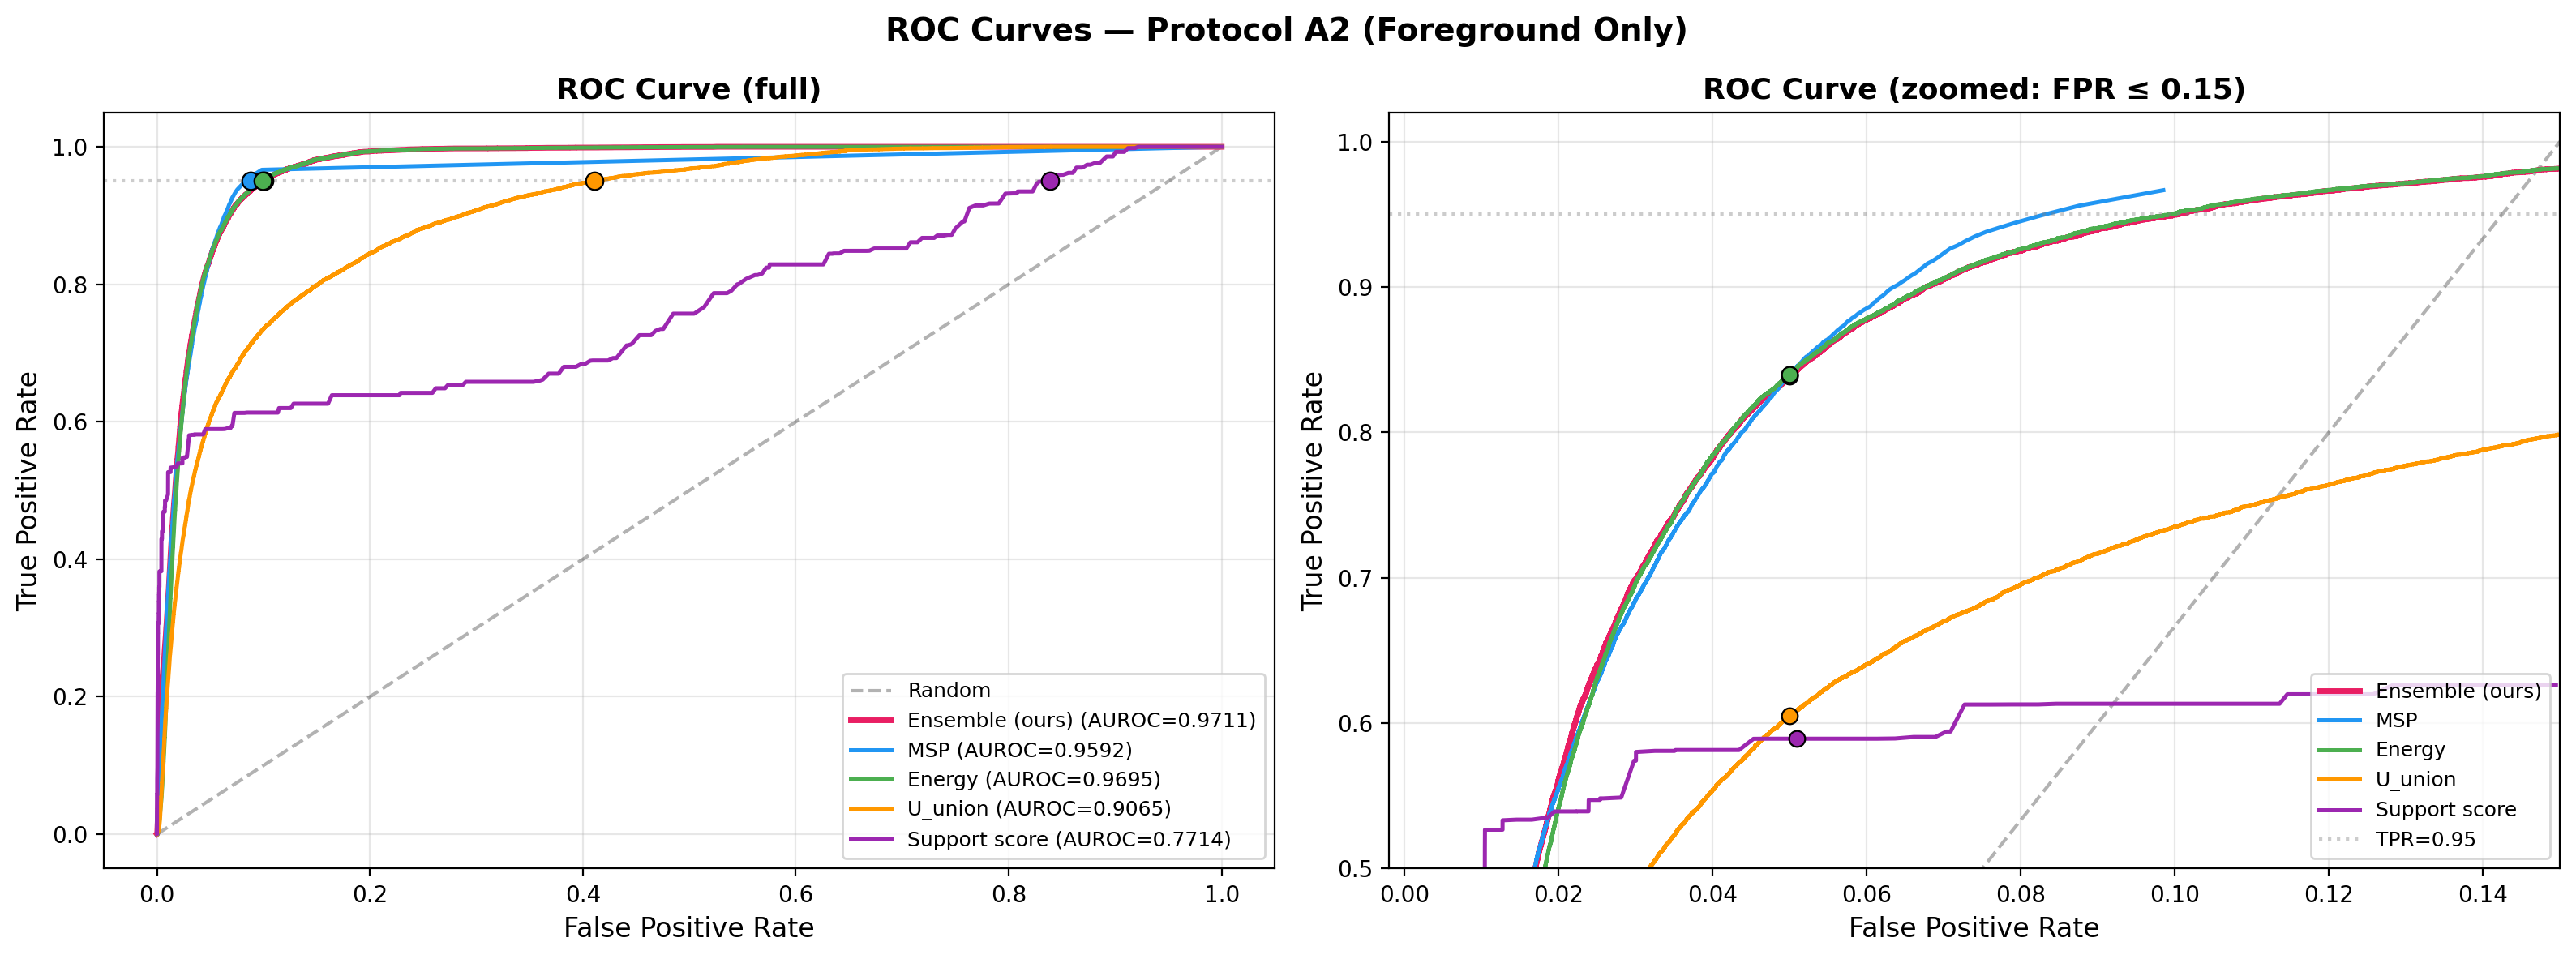
\includegraphics[width=\textwidth]{t3_roc_curve_a2.pdf}%
  }{%
    \IfFileExists{t3_roc_curve_a2.png}{%
      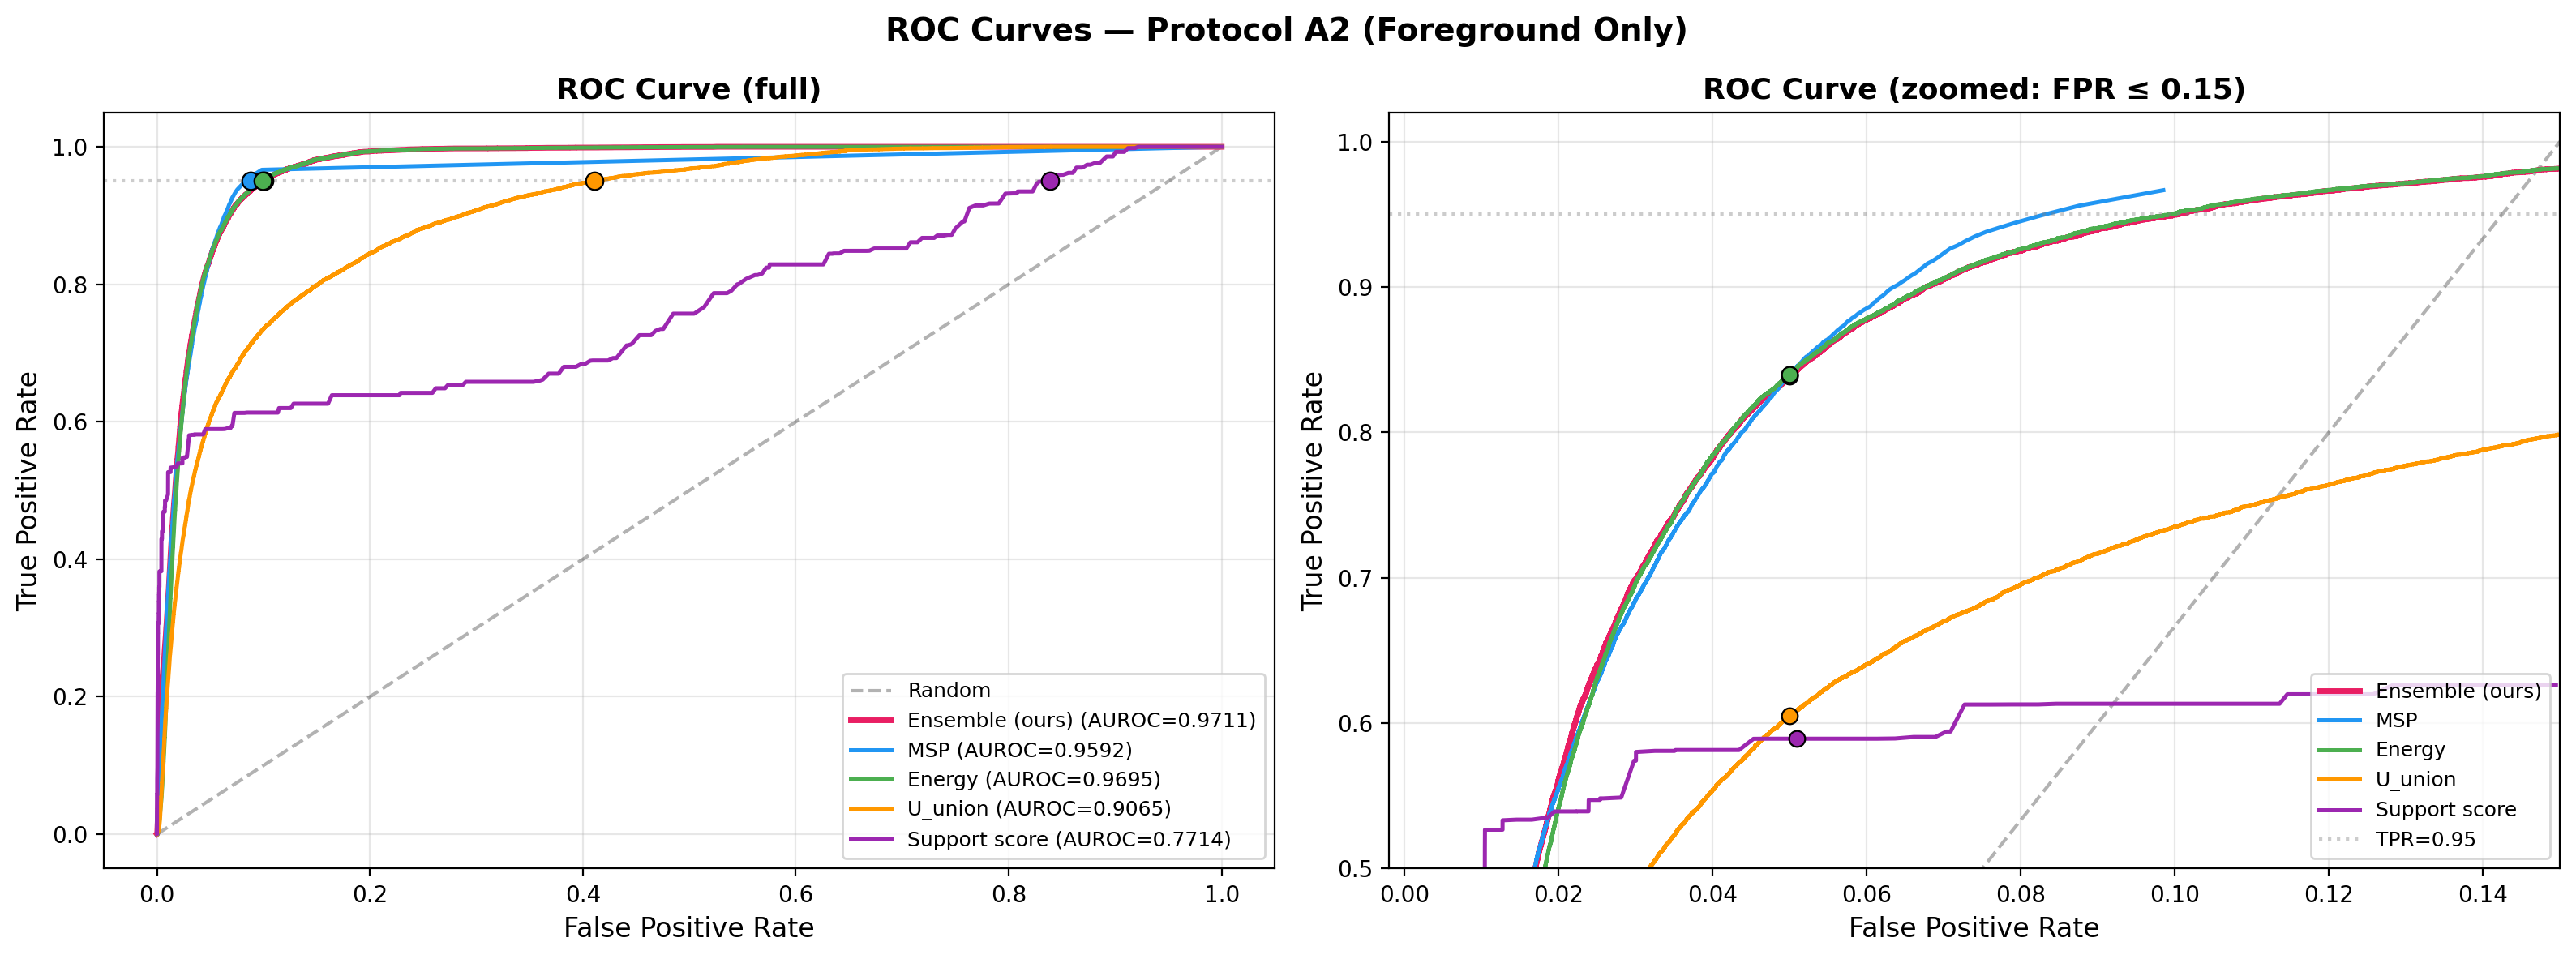
\includegraphics[width=\textwidth]{t3_roc_curve_a2.png}%
    }{%
      \fbox{\parbox{\textwidth}{\centering\vspace{4cm}ROC 占位\vspace{4cm}}}%
    }%
  }
  \caption{Synapse A2 协议下各 unknown 检测信号的 ROC 曲线（前景像素）。
  分类不确定性信号（MSP、Energy、Ensemble）在全局排序上显著优于几何支持分数（Support）。}\label{fig:a2_roc}
\end{figure*}

\begin{figure*}[!t]
  \centering
  \IfFileExists{t3_pr_curve_a2.pdf}{%
    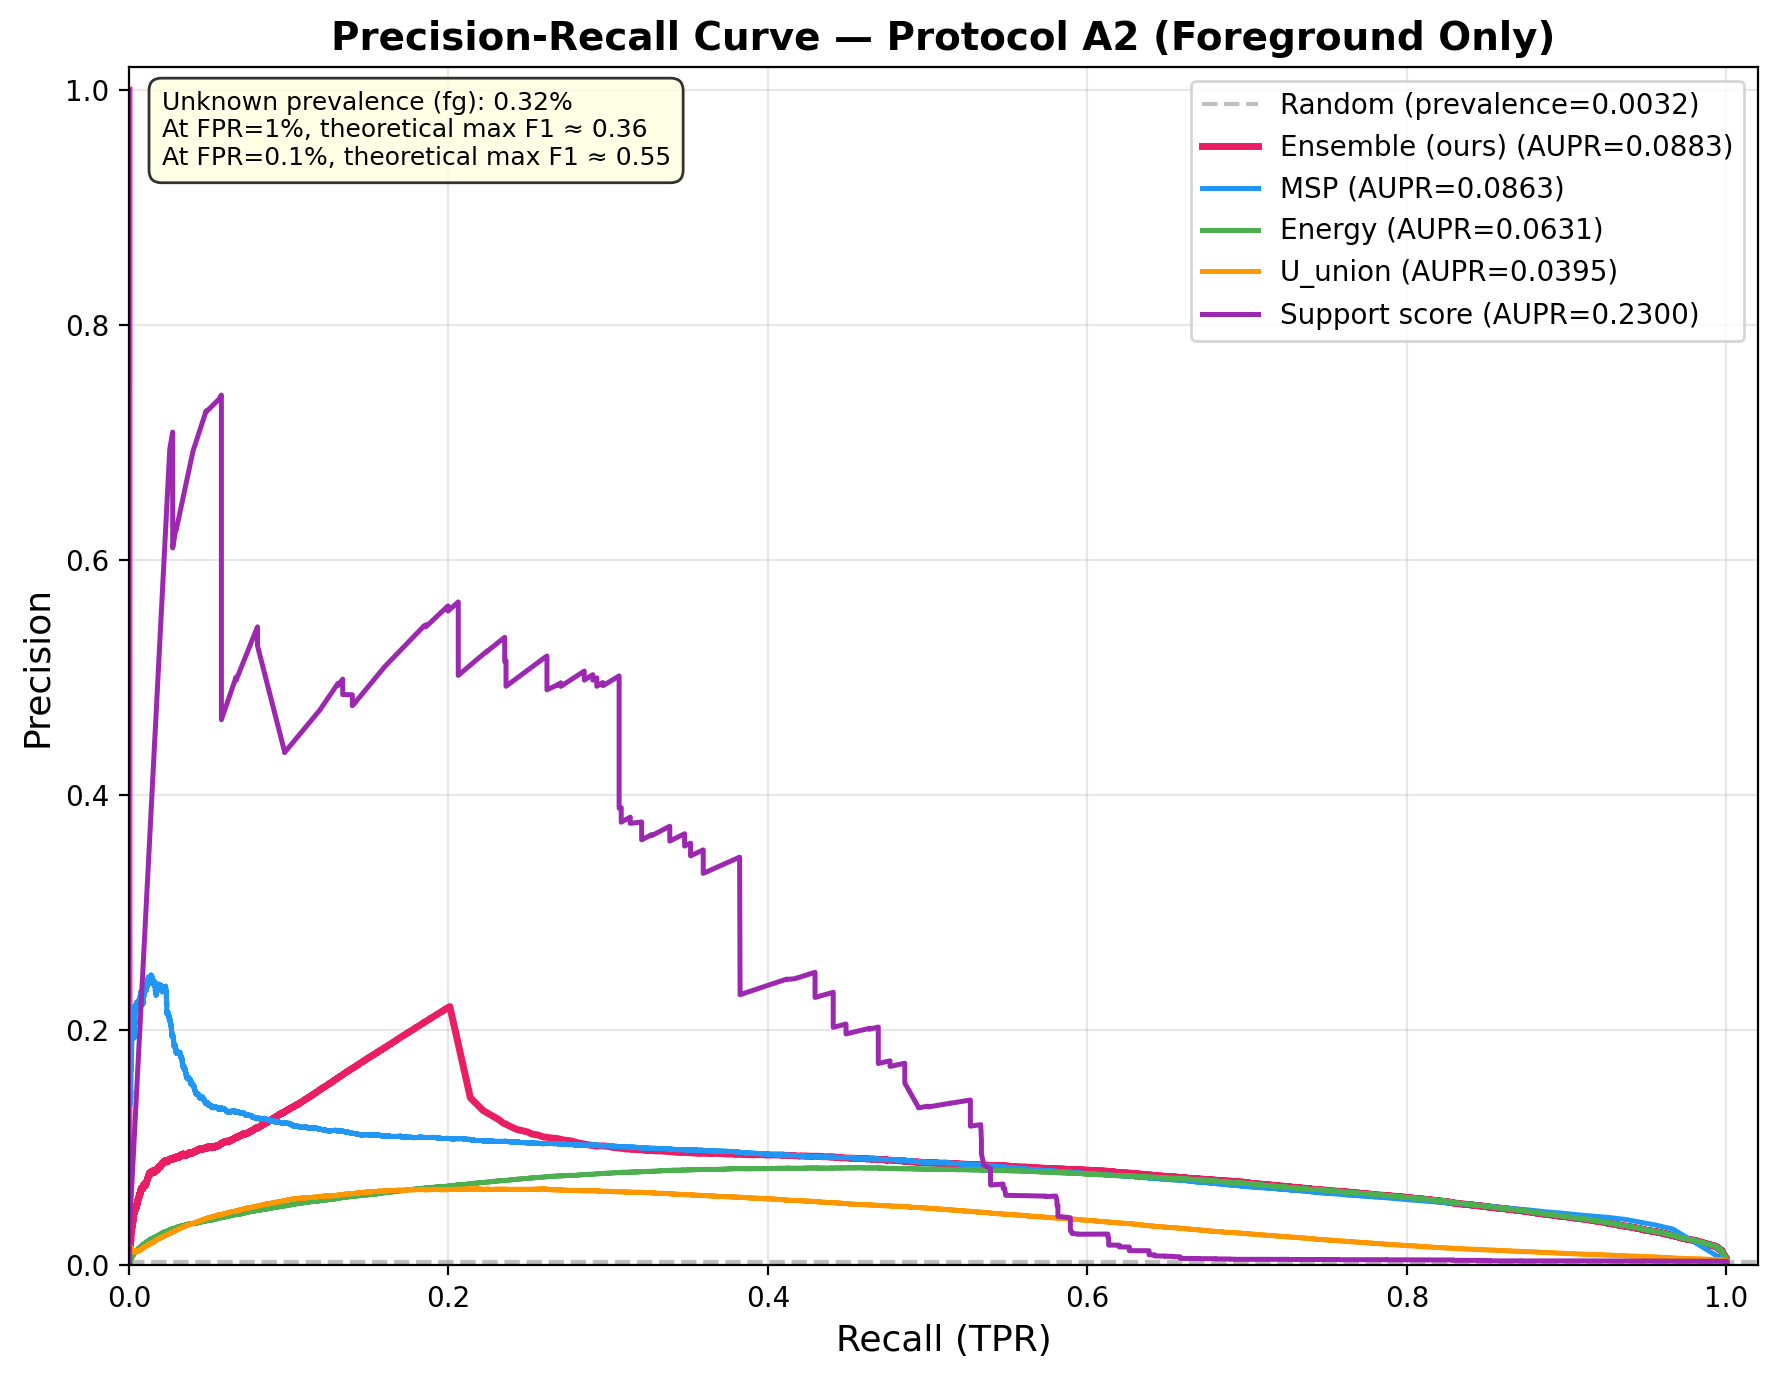
\includegraphics[width=\textwidth]{t3_pr_curve_a2.pdf}%
  }{%
    \IfFileExists{t3_pr_curve_a2.png}{%
      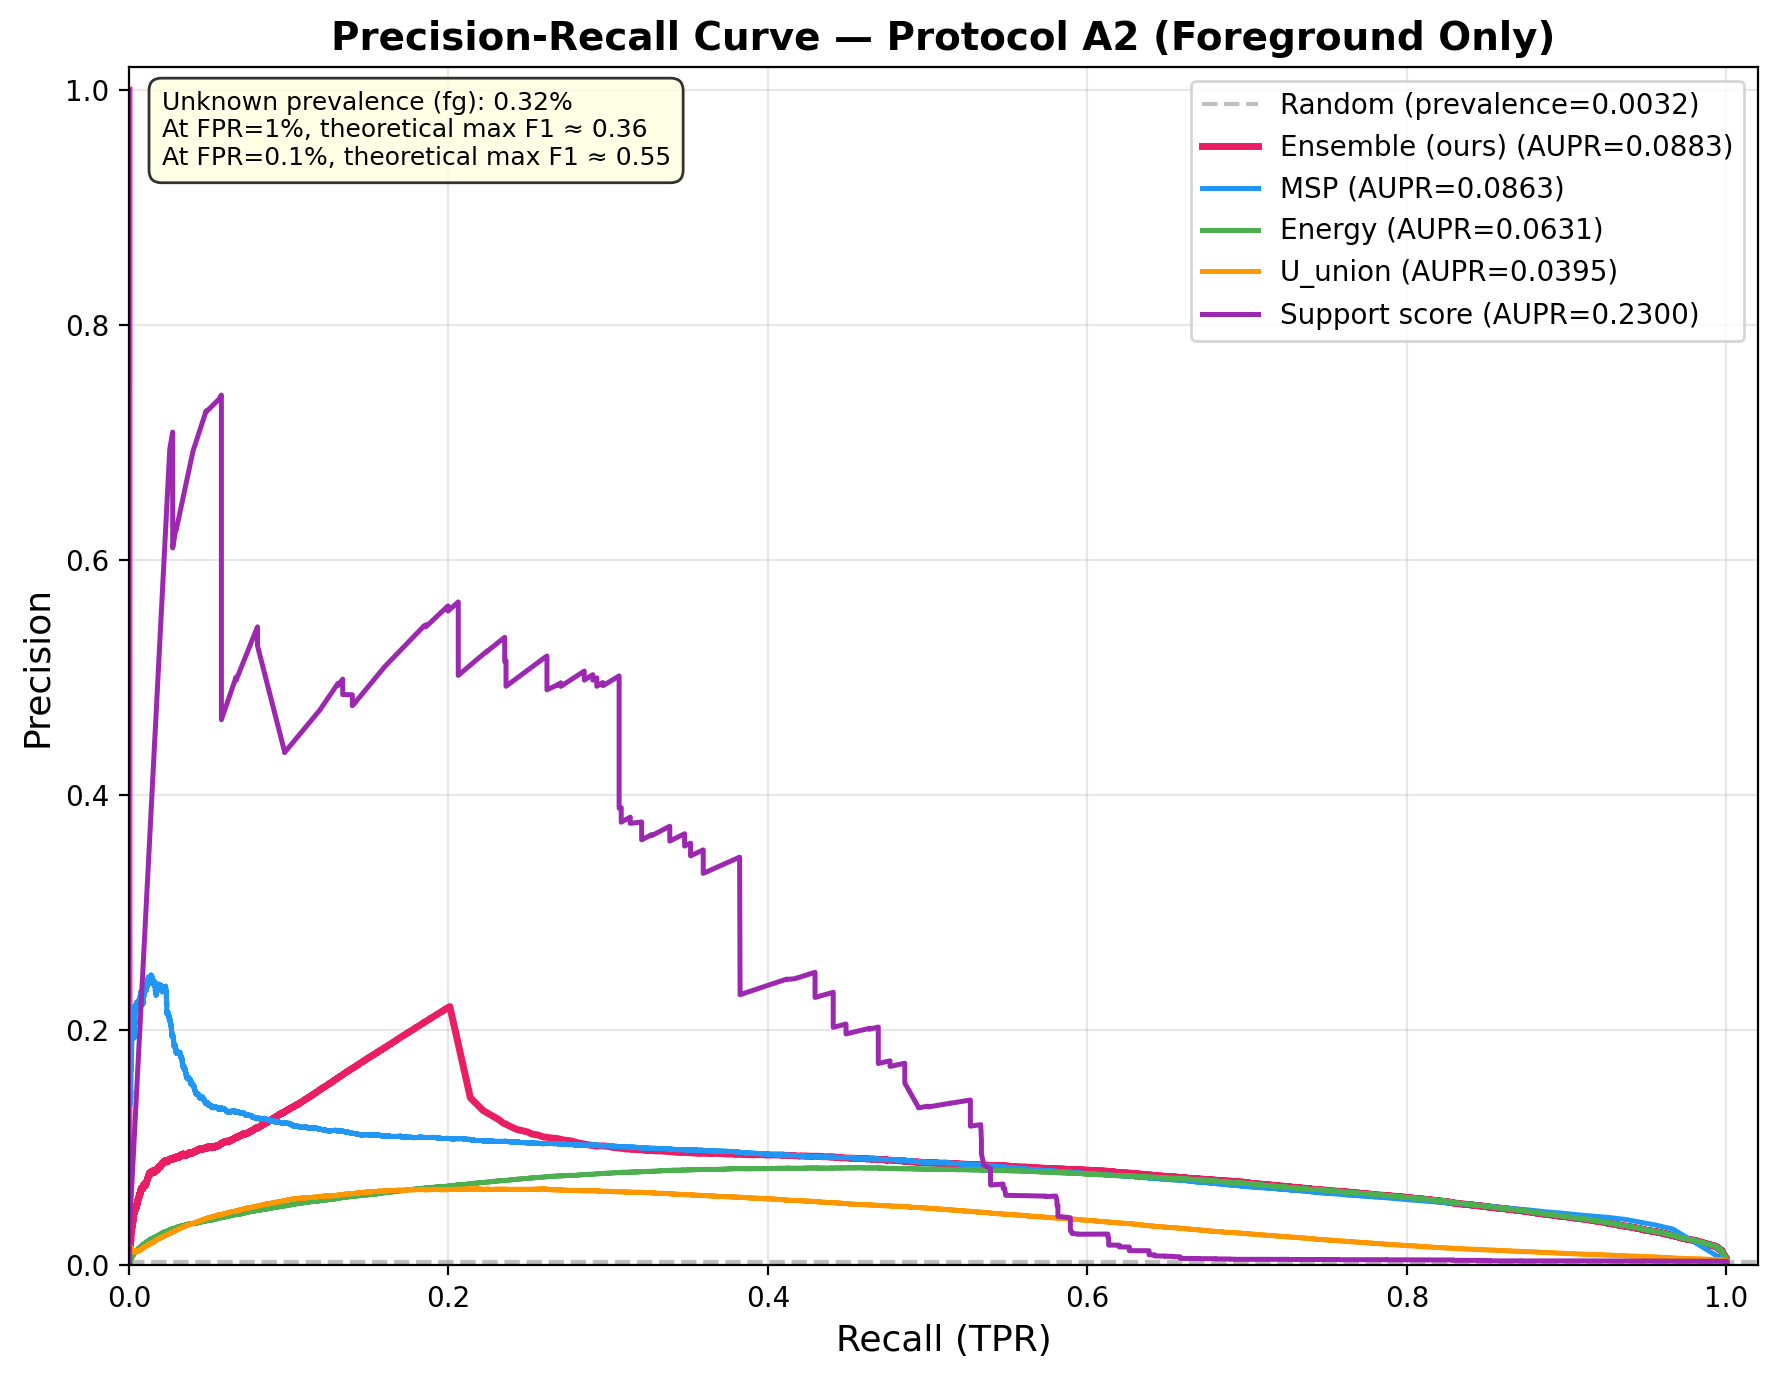
\includegraphics[width=\textwidth]{t3_pr_curve_a2.png}%
    }{%
      \fbox{\parbox{\textwidth}{\centering\vspace{4cm}PR 占位\vspace{4cm}}}%
    }%
  }
  \caption{Synapse A2 协议下各 unknown 检测信号的 Precision--Recall 曲线（前景像素）。
  Support 在高 precision 区间保留局部优势，但整体 AUPR 受限于全局排序能力。}\label{fig:a2_pr}
\end{figure*}


% ---------- 5.4 消融实验 ----------
\subsection{消融实验}\label{sec:exp:ablation}

\subsubsection{结构消融}\label{sec:exp:ablation:struct}

表~\ref{tab:ablation}~报告了在 Synapse A1 协议下，
逐项修改模型结构或损失函数的消融结果（单种子 seed=42）。

\begin{table}[t]
\centering
\footnotesize
\setlength{\tabcolsep}{4pt}
\caption{Synapse A1 结构消融。Baseline 为默认配置（$M=2, R=2$，完整损失，空对象机制开启）。
每行仅改变一个变量。}\label{tab:ablation}
\resizebox{\columnwidth}{!}{%
\begin{tabular}{lcc}
\toprule
设定 & Known mIoU & Unknown F1 \\
\midrule
Baseline（$M=2, R=2$） & $0.811$ & $0.721$ \\
\midrule
$M=1$ & $0.814$ & $0.697$ \\
$M=4$ & $0.810$ & $0.711$ \\
\midrule
$R=1$ & $0.800$ & $0.670$ \\
$R=4$ & $0.812$ & $0.713$ \\
\midrule
w/o $\mathcal{L}_{\text{ball}}$ & $0.797$ & $0.662$ \\
w/o $\mathcal{L}_{\text{boundary}}$ & $0.813$ & $0.724$ \\
w/o no-object & $0.814$ & $0.709$ \\
\bottomrule
\end{tabular}
}
\end{table}

关键发现如下。

\paragraph{Unknown slot 数量（$M$）}
$M=2$ 是最优配置（F1=0.721），$M=1$ 显著下降至 0.697（$-$2.4pp），
$M=4$ 无进一步提升（0.711）。
这说明两个 slot 已足以覆盖单张切片上 unknown 区域的空间多样性，
增加更多 slot 反而引入冗余。

\paragraph{原型球数量（$R$）}
$R=1$（单原型）导致 known mIoU 和 unknown F1 同时下降（mIoU $-$1.1pp，F1 $-$5.1pp），
$R=4$ 相对 $R=2$ 无明显改善。
这验证了 $R=2$ 对覆盖器官层位双峰分布的有效性。

\paragraph{损失函数}
去除 $\mathcal{L}_{\text{ball}}$ 导致 unknown F1 下降最大（$-$5.9pp），
同时 known mIoU 也下降 1.4pp，
表明几何约束不仅有助于 unknown 判定，还对已知类表示质量有间接促进作用。
去除 $\mathcal{L}_{\text{boundary}}$ 对 F1 影响甚微（+0.3pp），
同时 precision 从 0.775 升至 0.796、recall 从 0.674 降至 0.664，
说明该项在当前设置下主要改变 precision--recall 权衡，而非显著改变总体 F1。
去除 no-object 机制导致 F1 下降 1.2pp，影响温和。

\subsubsection{$M=0$ 核心消融：原生未知查询的必要性}\label{sec:exp:ablation:m0}

表~\ref{tab:m0}~报告了完全移除 unknown 查询（$M=0$）后的结果，
这是本文最核心的消融实验。

\begin{table}[t]
\centering
\footnotesize
\setlength{\tabcolsep}{3pt}
\caption{$M=0$ 消融：移除原生未知查询后，后处理信号能否替代结构化弃权？
Synapse A1 协议。表中的 \texttt{---} 表示该指标在该设定下不适用或未报告。}\label{tab:m0}
\resizebox{\columnwidth}{!}{%
\begin{tabular}{lccc}
\toprule
设定 & Known mIoU & Unknown F1 & AUROC$_{\text{fg}}$ \\
\midrule
$M=2$ + $U_{\text{union}}$ & $0.809$ & $\mathbf{0.728}$ & --- \\
$M=2$ + Support & $0.811$ & $0.721$ & --- \\
\midrule
$M=0$ + MSP & $0.782$ & $0.070$ & $0.965$ \\
$M=0$ + Prototype-sphere & $0.791$ & $0.008$ & $0.562$ \\
\bottomrule
\end{tabular}
}
\end{table}

结果具有决定性意义。
\textbf{移除 unknown 查询后，unknown F1 从 0.721--0.728 彻底崩塌至 0.008--0.070}
（降幅 $>$90\%），而 known mIoU 仅下降约 2\%。
值得注意的是，$M=0$ + MSP 的像素级 AUROC 仍高达 0.965，
说明后处理信号在像素级\textbf{排序}上仍然有效——
但它无法将这种排序能力转化为空间连贯的 unknown 掩码。

\textbf{这组消融直接说明：在本框架内部，移除 unknown 查询后，
仅依赖后处理信号不足以替代显式 unknown 输出空间。}
结合第~\ref{sec:exp:indep}~节的独立 baseline 比较可见，
A1 设定下真正关键的是是否为 unknown 保留原生输出空间，
而不只是具体采用 query-based 还是 per-pixel 的实现方式。

\paragraph{划分鲁棒性验证}
为检验上述结论是否依赖于特定的 seen/unseen 类别划分，
我们构造了一个替换划分（alt-split）：
将原始 unseen 侧的一个病理类（肝脏肿瘤，label 12）移至 seen 侧，
同时将原始 seen 侧的一个解剖类（胰腺，label 11）移至 unseen 侧，
从而刻意跨越原始划分的语义边界。
表~\ref{tab:alt_split}~对比了两种划分下的 $M=0$ 消融结果。

\begin{table}[t]
\centering
\footnotesize
\setlength{\tabcolsep}{3pt}
\caption{划分鲁棒性验证：替换 seen/unseen 划分后，$M=0$ 崩塌仍然成立。
Synapse A1 协议。}\label{tab:alt_split}
\begin{tabular}{llcc}
\toprule
划分 & 设定 & Known mIoU & Unknown F1 \\
\midrule
原始 & $M=2$（Support） & $0.811$ & $0.721$ \\
原始 & $M=0$（MSP） & $0.782$ & $0.070$ \\
\midrule
替换 & $M=2$（Support） & $0.819$ & $0.787$ \\
替换 & $M=0$（MSP） & $0.831$ & $0.043$ \\
\bottomrule
\end{tabular}
\end{table}

替换划分下，unknown F1 从 0.787 崩塌至 0.043（降幅 94.6\%），
甚至大于原始划分的 90.3\%，而 known mIoU 保持稳定。
这表明 $M=0$ 消融所揭示的机制——
移除 unknown 查询导致结构化弃权能力崩塌——
不依赖于特定的类别划分方式。

图~\ref{fig:m0_vis}~展示了 $M=2$ 与 $M=0$ 的定性对比。
$M=2$ 模型在 unknown 区域产生连贯的分割掩码，
而 $M=0$ 模型的后处理结果呈现碎片化、无法形成有意义的区域。

\begin{figure*}[!t]
  \centering
  \IfFileExists{t2_m2_vs_m0_grid.pdf}{%
    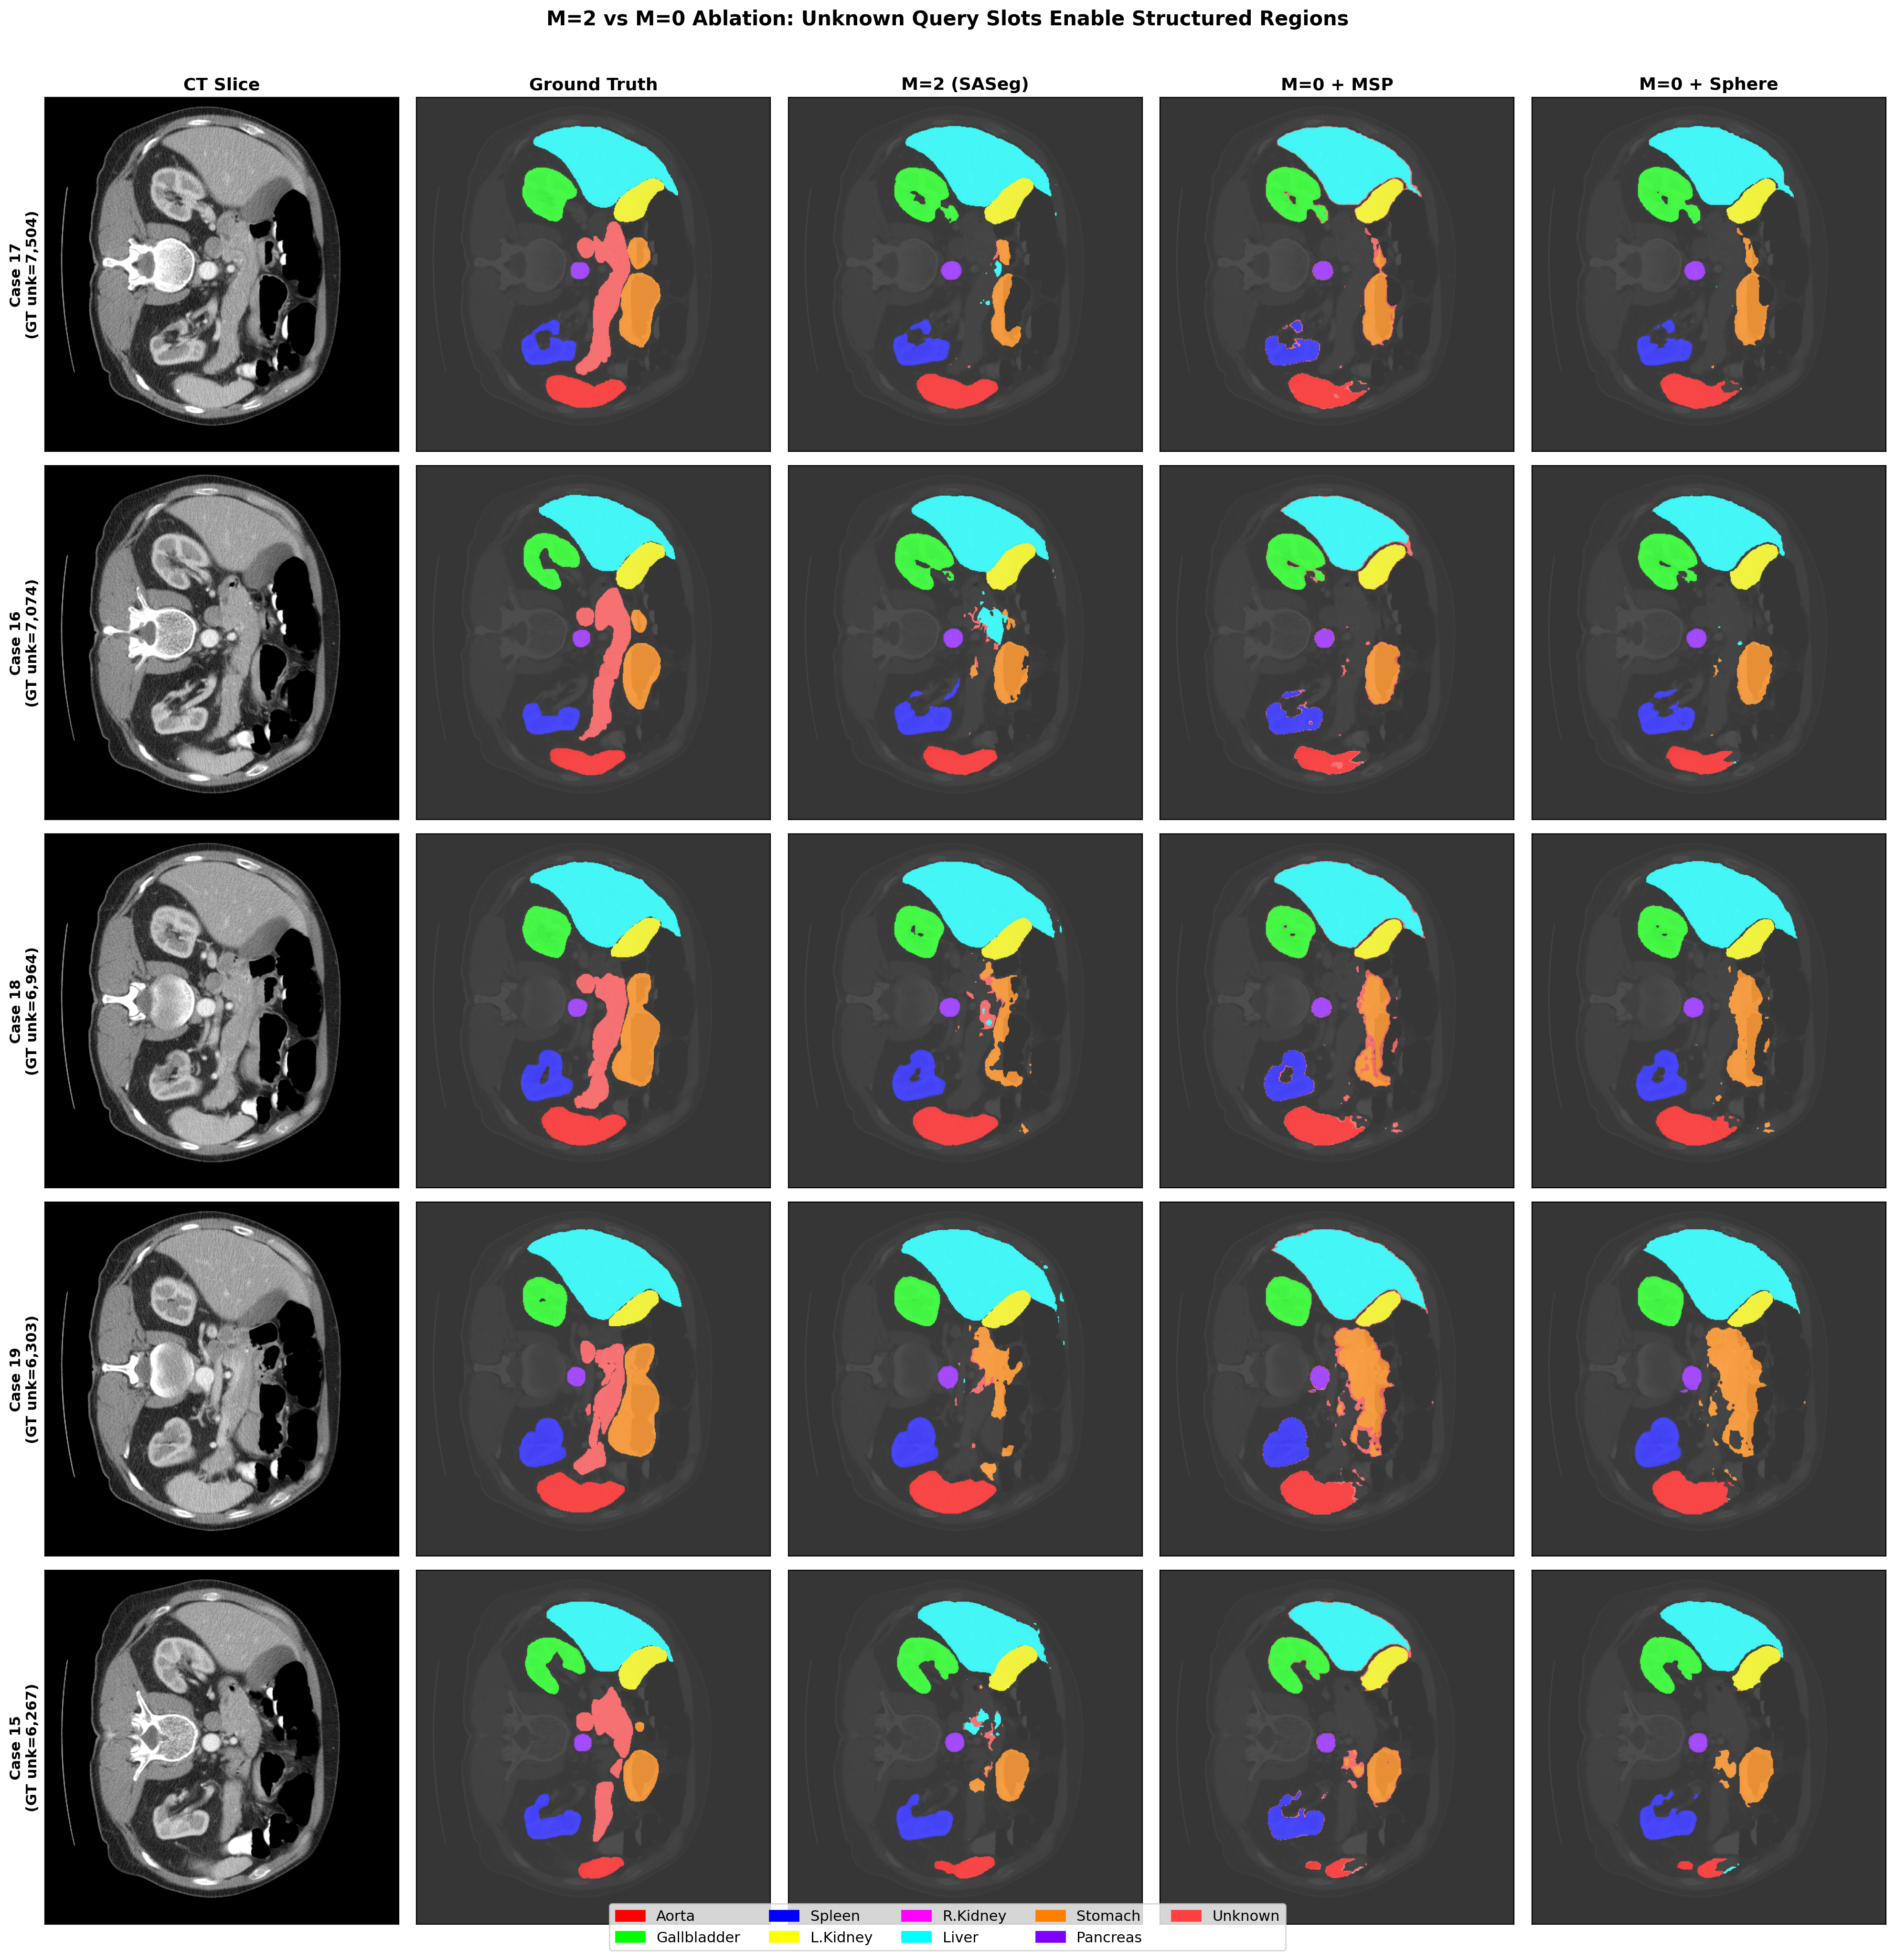
\includegraphics[width=\textwidth]{t2_m2_vs_m0_grid.pdf}%
  }{%
    \IfFileExists{t2_m2_vs_m0_grid.png}{%
      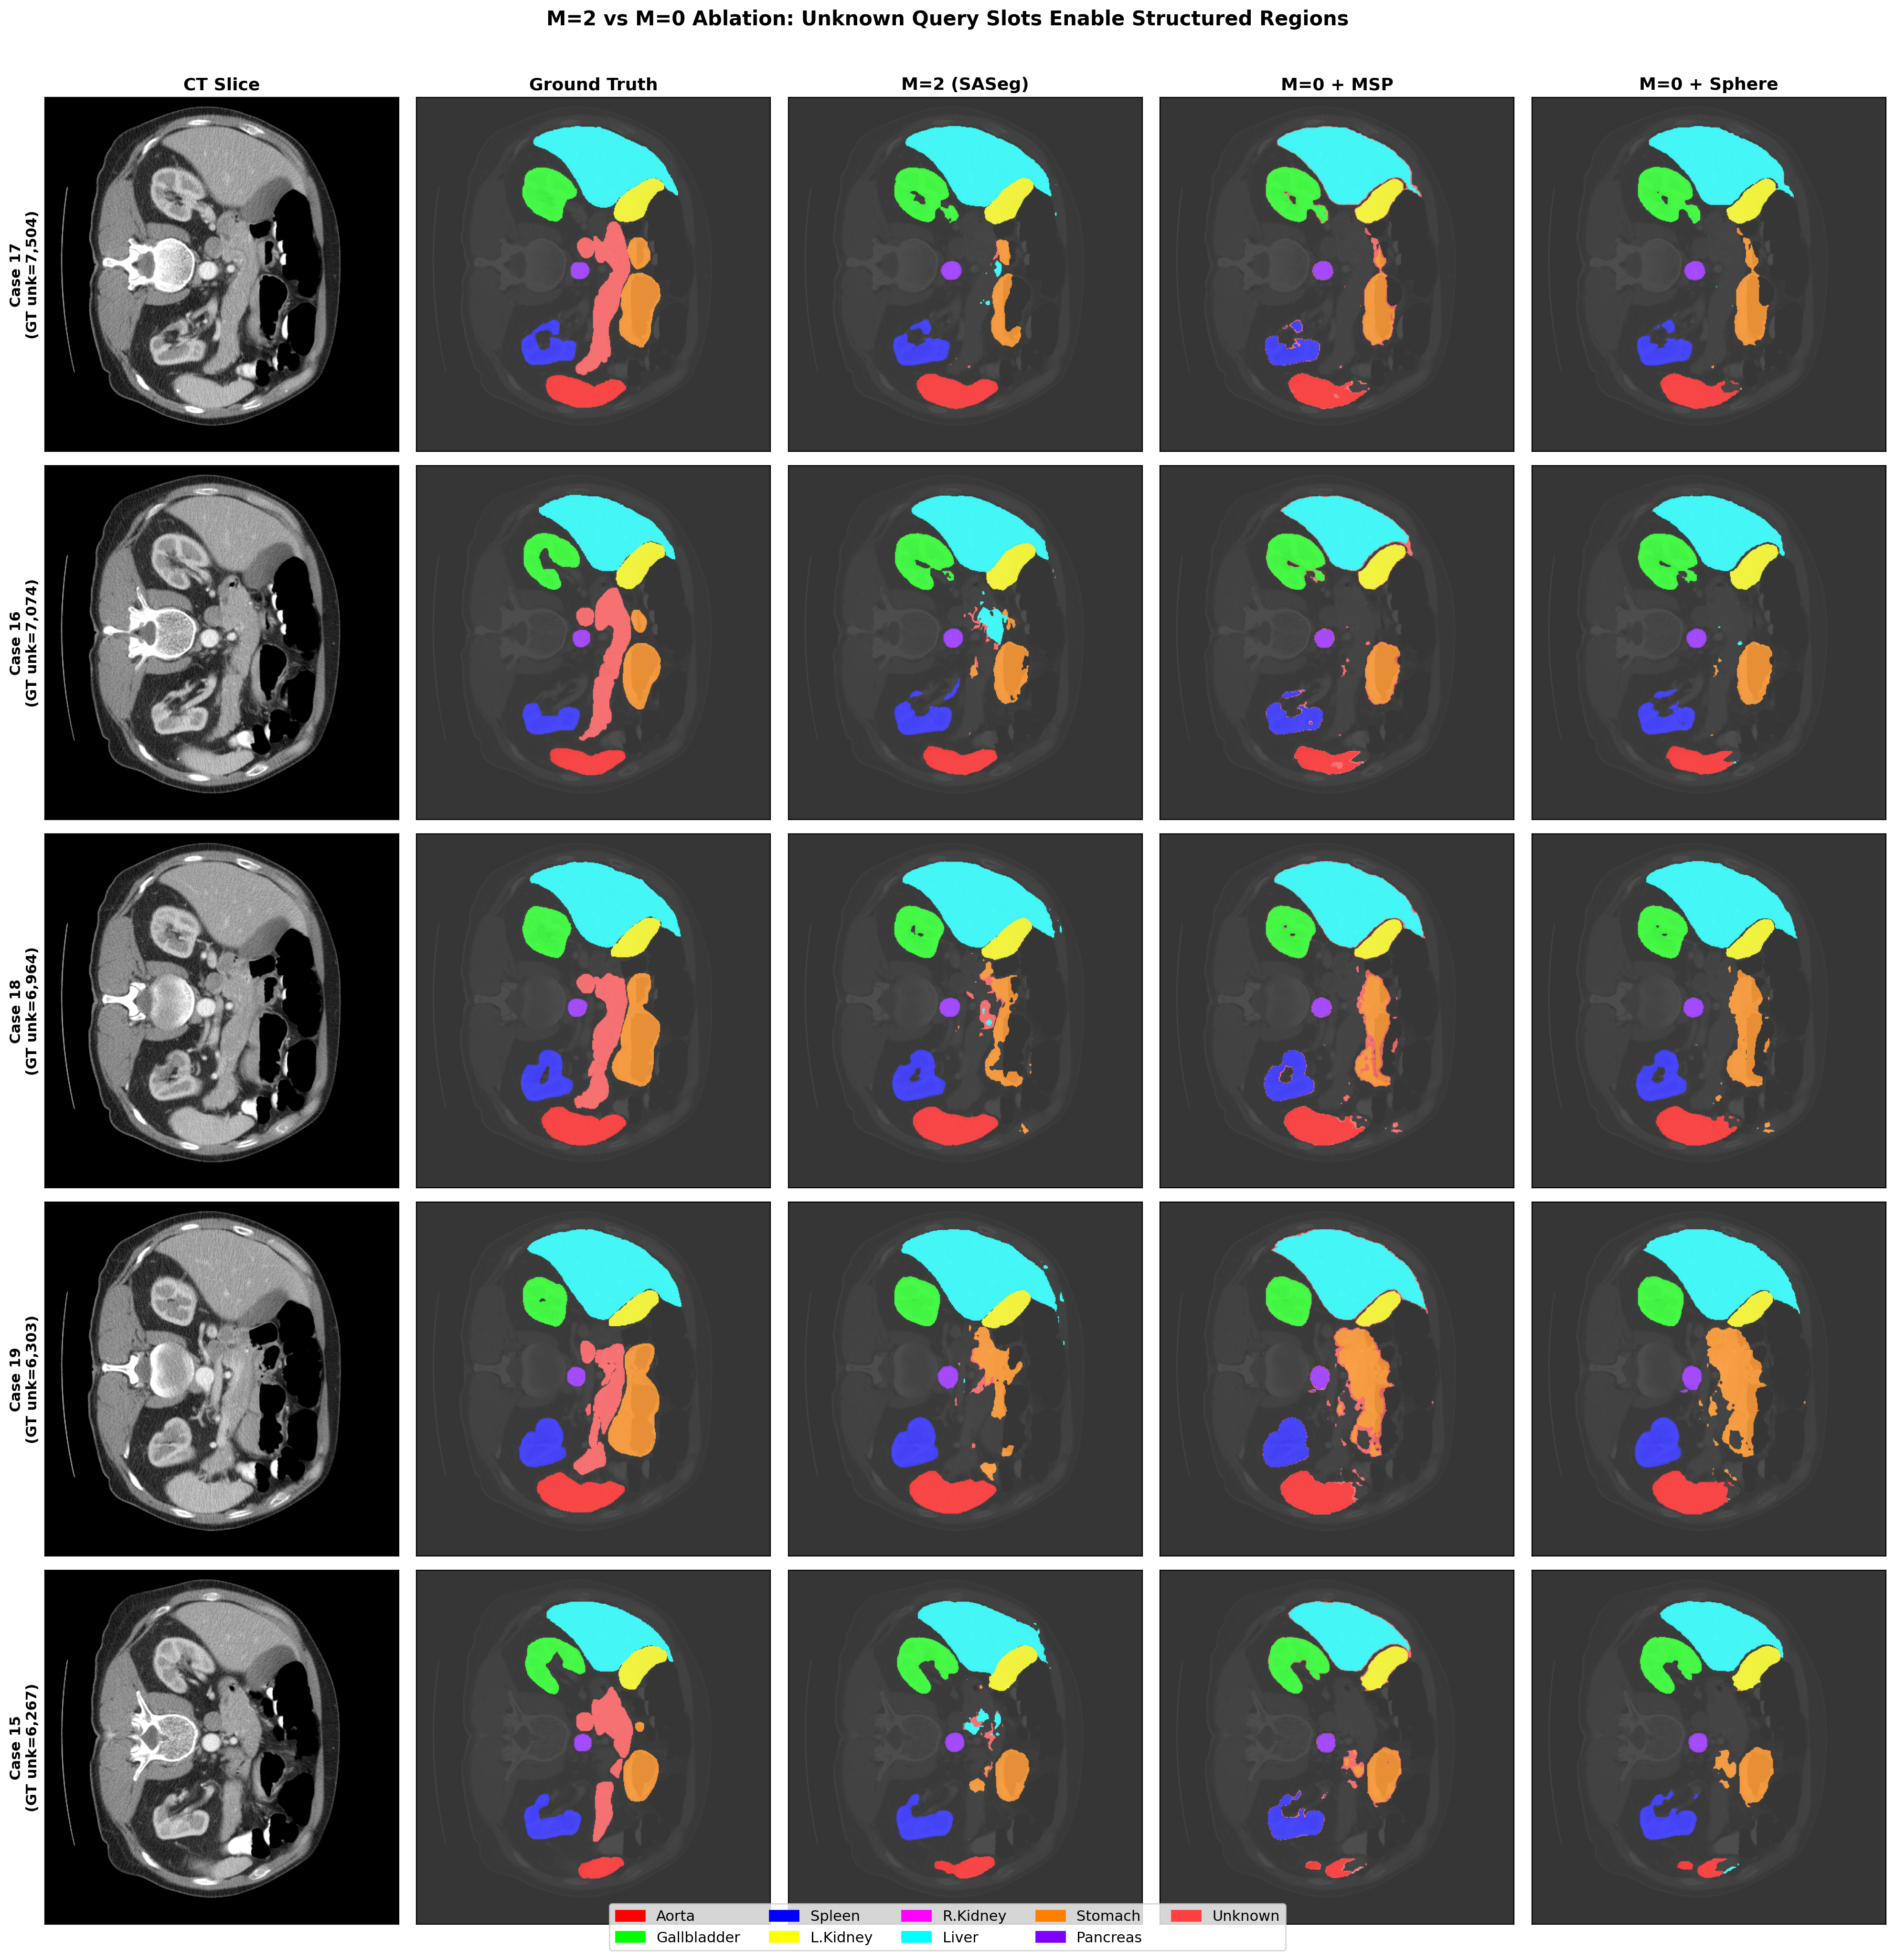
\includegraphics[width=\textwidth]{t2_m2_vs_m0_grid.png}%
    }{%
      \fbox{\parbox{\textwidth}{\centering\vspace{4cm}$M=2$ vs $M=0$ 定性对比占位\vspace{4cm}}}%
    }%
  }
  \caption{$M=2$（上）与 $M=0$（下）在 Synapse A1 上的定性对比。
  $M=2$ 模型通过原生未知查询产生空间连贯的 unknown 掩码（红色），
  而 $M=0$ 模型的后处理 unknown 判定呈现碎片化分布，
  无法形成结构化的弃权输出。}\label{fig:m0_vis}
\end{figure*}


% ---------- 5.5 跨数据集验证 ----------
\subsection{跨数据集验证：AMOS22}\label{sec:exp:cross}

为验证核心结论的跨数据集一致性，
我们在 AMOS22 CT 子集上复现了三项关键实验：A1、A2 与 $M=0$ 消融。
其中采用 CT-only 设置，带标注的 CT 训练集与验证集分别为 200 例和 100 例；
AMOS22 上的结果来自独立训练后的验证集评估，而非仅将其作为 validation split 使用。
AMOS22 包含 15 类器官标注，按 $K=8$（已知）/ 4（seen unknown）/ 3（unseen unknown）划分。

表~\ref{tab:cross}~汇总了跨数据集对比结果。

\begin{table*}[!t]
\centering
\caption{Synapse 与 AMOS22 的跨数据集对比。
三项核心结论在两个独立数据集上均保持一致。表中的 \texttt{---} 表示该指标在该设定下不适用或未报告。}\label{tab:cross}
\footnotesize
\resizebox{\textwidth}{!}{%
\begin{tabular}{ll ccc cc c}
\toprule
实验 & 数据集 & mIoU$_{\text{K}}$ & F1$_{\text{U}}$ & IoU$_{\text{U}}$ & Prec$_{\text{U}}$ & Rec$_{\text{U}}$ & AUROC$_{\text{fg}}$ \\
\midrule
\multirow{2}{*}{A1} & Synapse & $0.811$ & $0.721$ & $0.564$ & $0.775$ & $0.674$ & --- \\
                     & AMOS22  & $0.838$ & $0.839$ & $0.723$ & $0.848$ & $0.831$ & --- \\
\midrule
\multirow{2}{*}{A2 (Ens.)} & Synapse & $0.797$ & $0.006$ & $0.003$ & --- & --- & $0.971$ \\
                            & AMOS22  & $0.827$ & $0.010$ & $0.005$ & $0.006$ & $0.025$ & $0.990$ \\
\midrule
\multirow{2}{*}{$M\!=\!0$+MSP} & Synapse & $0.782$ & $0.070$ & --- & --- & --- & $0.965$ \\
                                 & AMOS22  & $0.814$ & $0.045$ & $0.023$ & $0.059$ & $0.037$ & $0.983$ \\
\multirow{2}{*}{$M\!=\!0$+Sph.} & Synapse & $0.791$ & $0.008$ & --- & --- & --- & $0.562$ \\
                                  & AMOS22  & $0.816$ & $0.017$ & $0.009$ & $0.077$ & $0.010$ & $0.780$ \\
\bottomrule
\end{tabular}%
}
\end{table*}

三项核心结论均跨数据集成立：

\paragraph{A1 结构化弃权有效}
AMOS22 A1 的 unknown F1 达到 0.839，甚至高于 Synapse（0.711），
同时 known mIoU 保持 0.838。
这说明本框架的结构化弃权能力在更大规模数据集上不仅保持有效，甚至表现更强。

\paragraph{A2 中 detection $\neq$ structuring}
AMOS22 A2 的 Ensemble AUROC$_{\text{fg}}$ 高达 0.990（Synapse 为 0.971），
但 unknown F1 仅为 0.010，与 Synapse 的趋势完全一致。
这证明"高检测排序 $\neq$ 可用的结构化弃权输出"不是 Synapse 的偶然现象，
而是 unseen-unknown 场景下的固有特征。

\paragraph{$M=0$ 消融跨数据集确认}
在 AMOS22 上，移除 unknown 查询后 F1 从 0.839 崩塌至 0.045（MSP）/ 0.017（Sphere），
降幅分别为 94.6\% 和 98.0\%，与 Synapse 方向完全一致。
原生未知查询对结构化弃权的必要性在两个独立数据集上得到验证。


% ---------- 5.6 深入分析 ----------
\subsection{深入分析}\label{sec:exp:analysis}

\subsubsection{两类 Unknown Regime 的分布证据}\label{sec:exp:analysis:dist}

图~\ref{fig:score_dist}~展示了 support score 与 neg-maxprob 在 A1 和 A2 上的分布对比。

\begin{figure*}[!t]
  \centering
  \IfFileExists{t1_support_a1_vs_a2.pdf}{%
    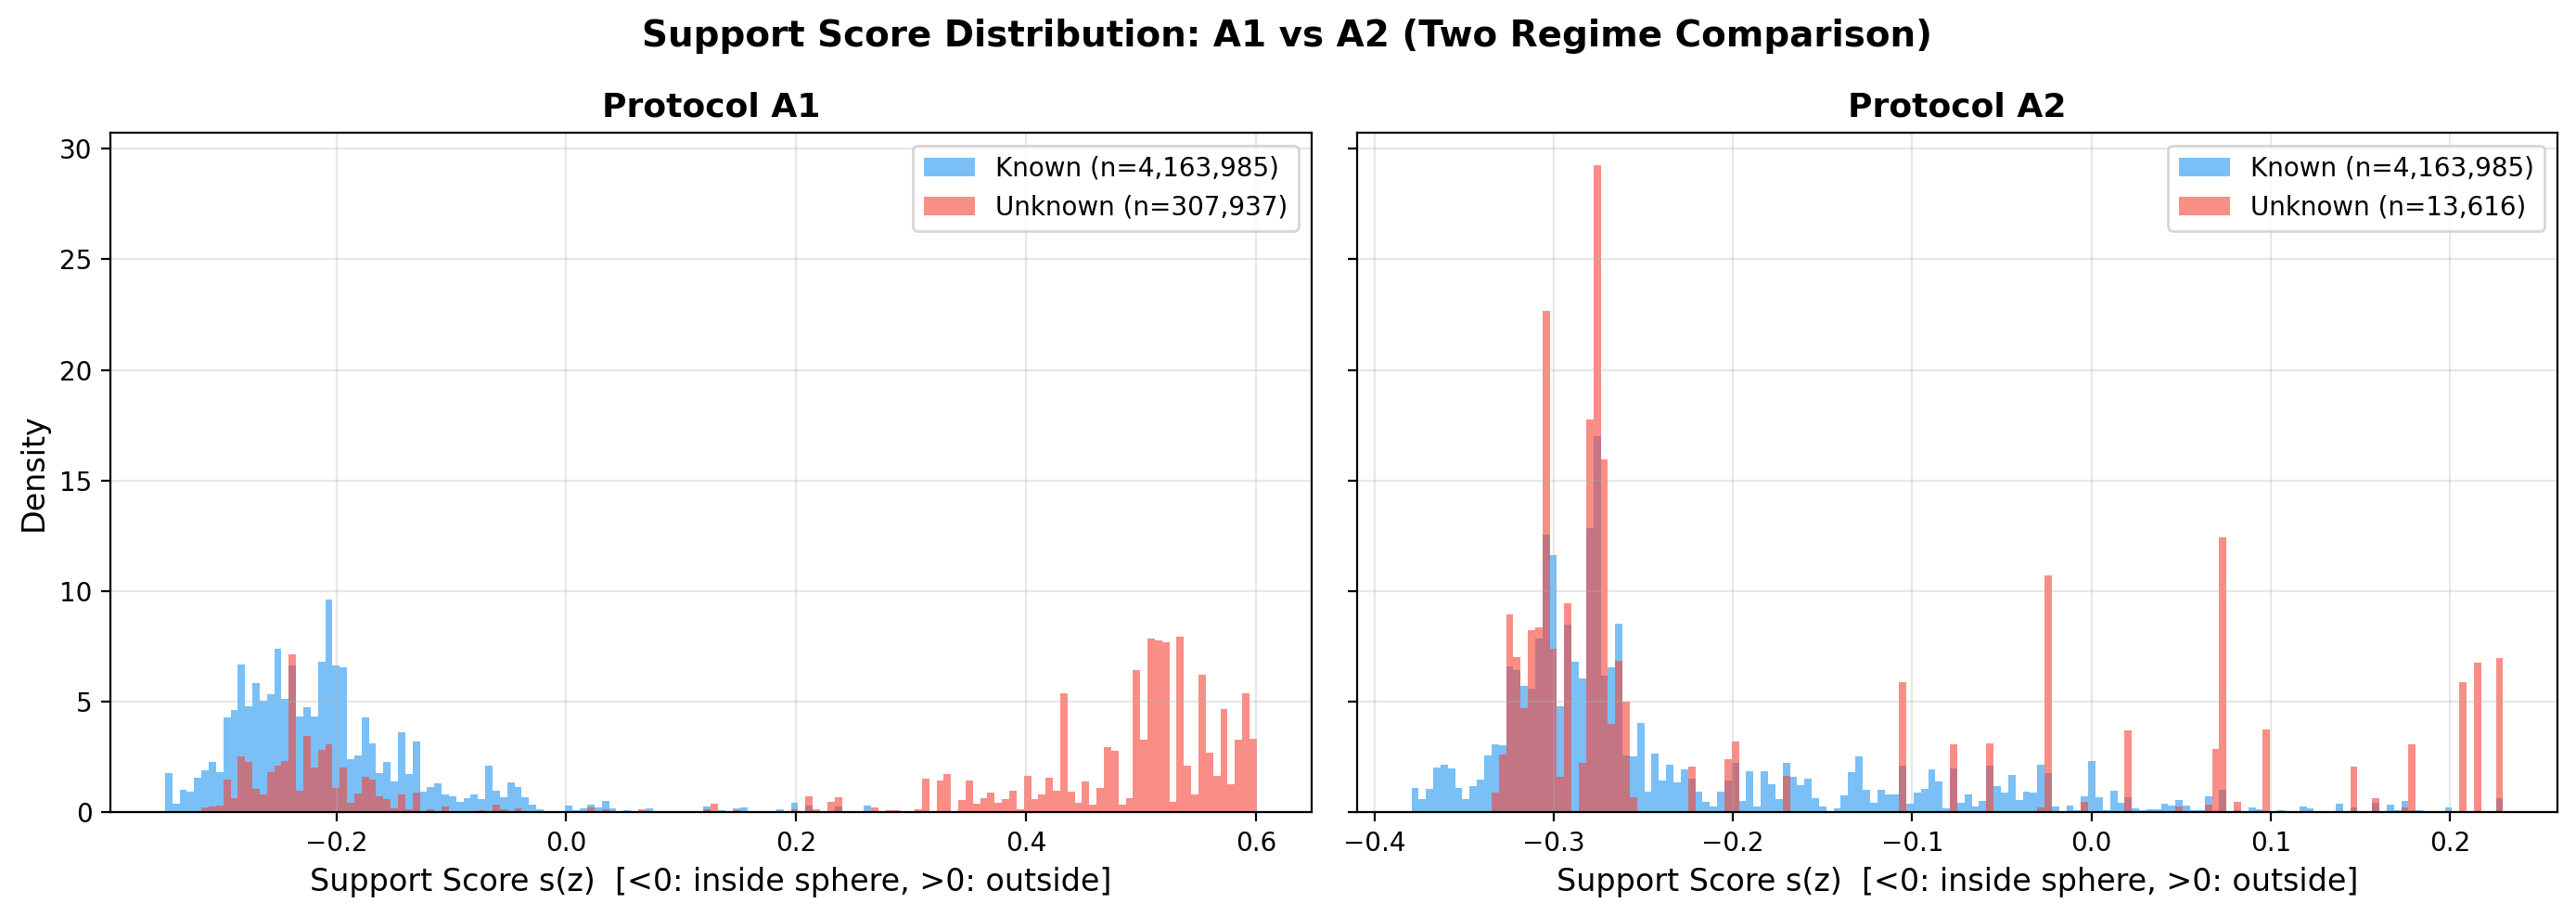
\includegraphics[width=\textwidth]{t1_support_a1_vs_a2.pdf}%
  }{%
    \IfFileExists{t1_support_a1_vs_a2.png}{%
      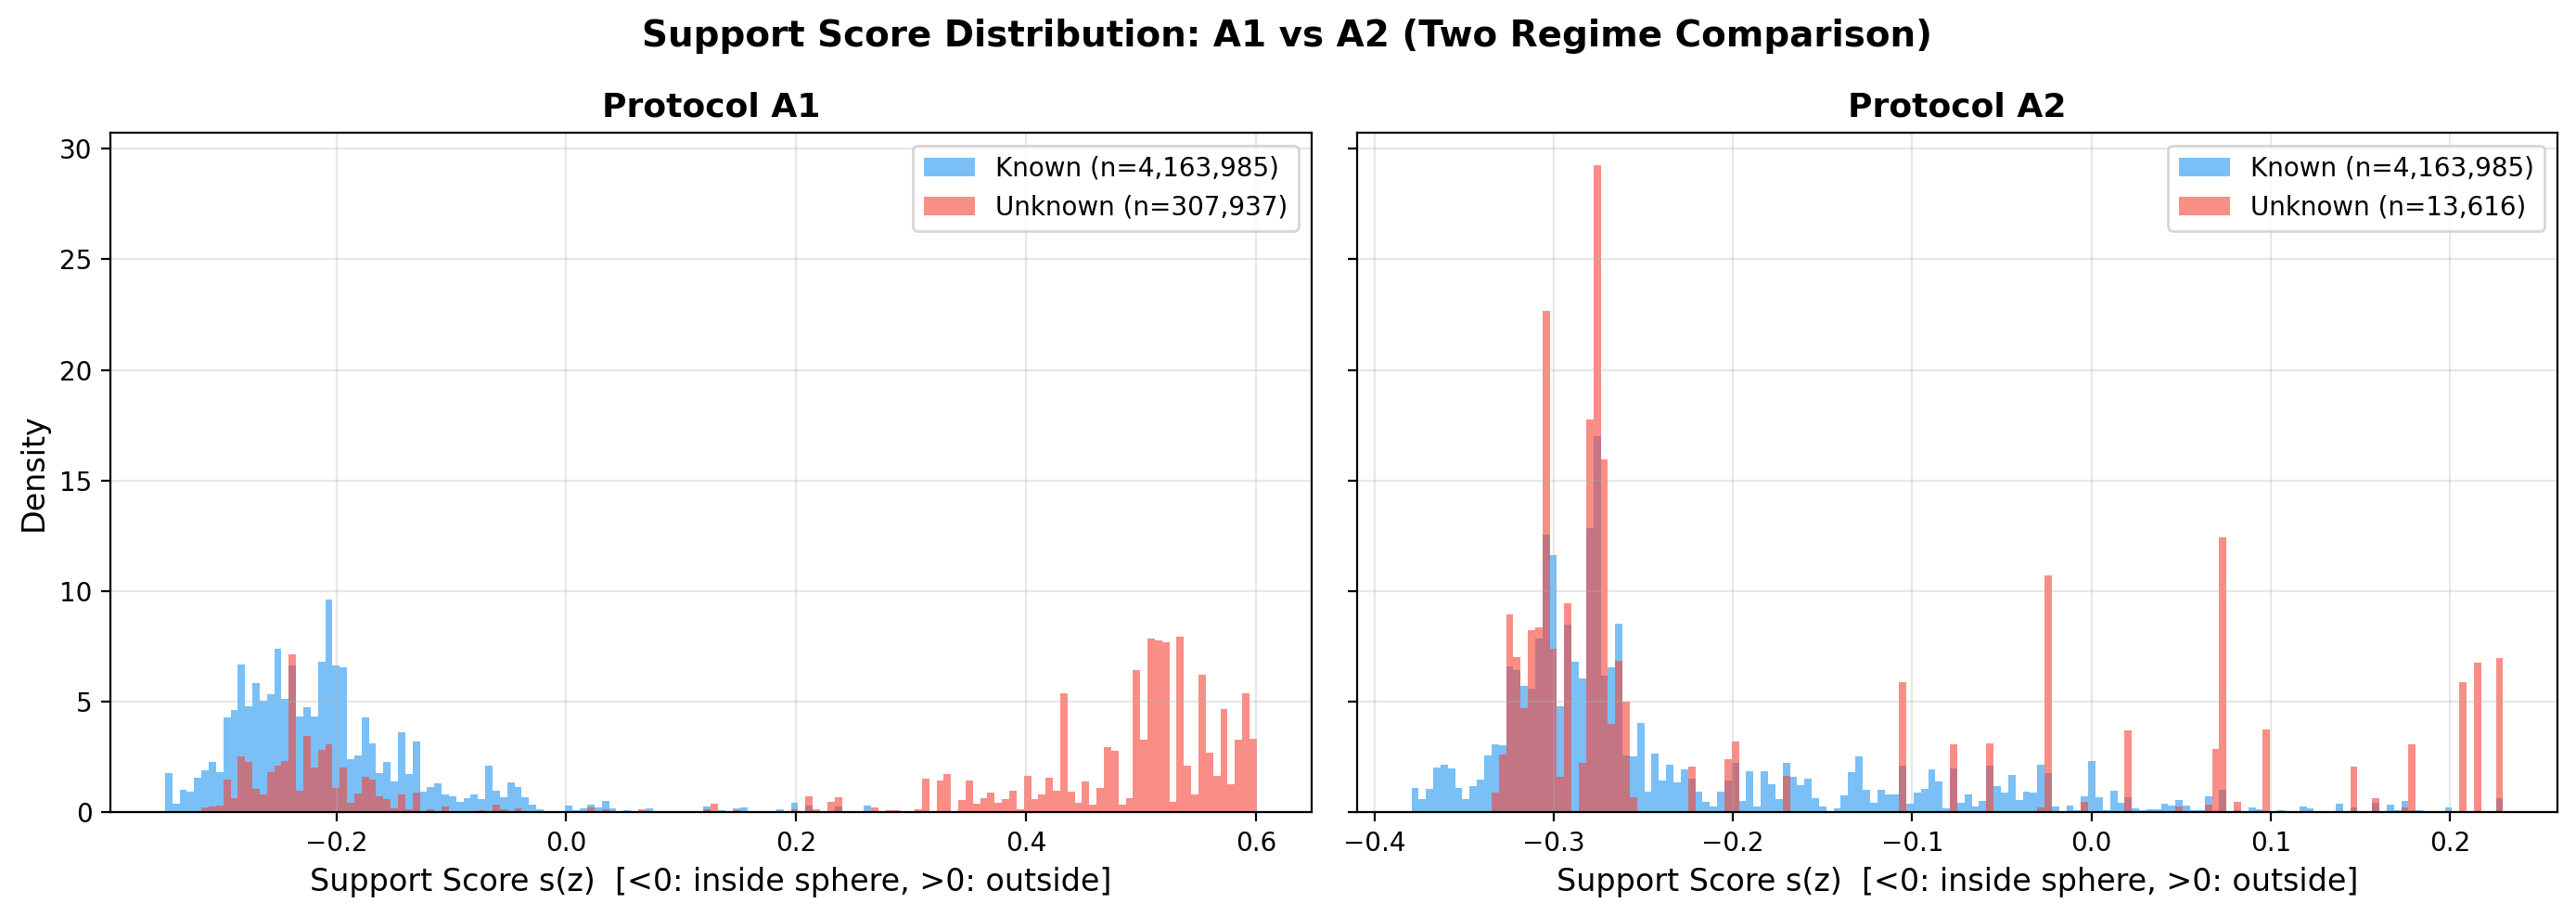
\includegraphics[width=\textwidth]{t1_support_a1_vs_a2.png}%
    }{%
      \fbox{\parbox{\textwidth}{\centering\vspace{3cm}Support score 分布对比占位\vspace{3cm}}}%
    }%
  }
  \caption{Support score 在 A1（左）与 A2（右）上的 known/unknown 分布对比。
  A1 中 known 与 unknown 的 support score 分布分离清晰（support-deficit regime），
  而 A2 中二者大量重叠（competitive-ambiguity regime），
  解释了 support score 在 A2 上排序能力受限的原因。}\label{fig:score_dist}
\end{figure*}

在 A1（support-deficit regime）中，
unknown 区域的 support score 显著高于 known 区域，两类分布清晰分离，
support score 可有效区分二者。
在 A2（competitive-ambiguity regime）中，
unseen unknown 与 known 的 support score 分布大量重叠，
因为 unseen unknown 在特征空间中与某些已知类视觉相近，
其 embedding 落在已知类原型球附近甚至内部，导致 support score 失效。
这一分布证据直观解释了为何 A2 需要切换到分类不确定性信号（表~\ref{tab:a2_main}），
也验证了双协议拆分的必要性——两类 unknown regime 由本质不同的信号主导。

\subsubsection{A2 Retrieval 分析}\label{sec:exp:analysis:retrieval}

第~\ref{sec:exp:a2}~节观察到 A2 的 Ensemble AUROC 很高但 F1 接近于零。
为理解这一现象，
表~\ref{tab:retrieval}~从 retrieval 视角分析 A2 的 ensemble 排序质量。
在 A2 前景像素中，unknown prevalence 仅为 0.32\%。

\begin{table}[t]
\centering
\caption{Synapse A2 top-$r$\% retrieval 分析（ensemble score 排序）。
Lift 为相对于随机 baseline 的富集倍数。}\label{tab:retrieval}
\begin{tabular}{lcccc}
\toprule
Budget & Precision & Recall & FPR & Lift \\
\midrule
top-0.1\% & $0.100$ & $0.031$ & $0.001$ & $30.8\times$ \\
top-0.3\% & $0.209$ & $0.193$ & $0.002$ & $64.3\times$ \\
top-0.5\% & $0.201$ & $0.310$ & $0.004$ & $62.0\times$ \\
top-1.0\% & $0.123$ & $0.380$ & $0.009$ & $38.0\times$ \\
\bottomrule
\end{tabular}
\end{table}

结果表明，ensemble 排序相对于随机 baseline 具有显著的富集效应
（top-0.3\% 时 lift=$64.3\times$），
但即便放宽到 top-1\%，recall 也仅为 0.380、precision 仅为 0.123。
这说明 A2 的 detection 信号具备明确的 retrieval 价值，
但这种排序能力\textbf{尚不足以}直接转化为高质量的结构化弃权掩码。

\subsubsection{A2 区域级候选分析}\label{sec:exp:analysis:region}

为进一步诊断 A2 结构化弃权失败的瓶颈，
我们对 unknown 查询生成的候选区域进行了区域级分析。
在 A2 的 50 张含 unseen unknown 的切片上：

\begin{itemize}[nosep]
  \item 66\% 的 unknown 切片至少有一个候选区域与 GT 存在重叠；
  \item 但 IoU$\geq$0.10 的 unknown-slice 命中率仅为 2\%；
  \item 对 $\geq$32 像素的较大连通域，IoU$\geq$0.10 命中率为 0\%；
  \item 候选区域总像素 253,365，而 GT unknown 总像素仅 13,616，
        candidate union IoU 均值仅 0.005。
\end{itemize}

这组结果揭示了 A2 结构化弃权的真正瓶颈：
\textbf{问题不在于最后一步 decision，而在于 candidate generation 本身。}
unknown 查询在 A2 下虽然会产生粗略响应，
但生成的候选区域与 GT 几乎没有有意义的空间对齐
（union IoU$=$0.005，IoU$\geq$0.10 接近于零）。
因此，即使使用完美的 region-level classifier 也无法从这些候选中恢复有效的 unknown 掩码。
这一发现将 A2 的 structuring 瓶颈从"如何做 decision"转移到了更根本的"如何生成纯净候选"，
为未来研究指出了方向。


\subsection{候选纯净度瓶颈的缓解探索}\label{sec:exp:explore}

第~\ref{sec:exp:analysis}节的分析揭示，A2 结构化弃权的根本瓶颈在于 candidate generation 本身，而非 decision 阶段。
为进一步精确化这一瓶颈的性质，我们沿两条独立路径展开了探索性实验。

\textbf{路径一：Known-Exclusion Loss。}
一个直观假设是：unknown 候选对已知类区域的侵入是纯净度低的主因，
因此可以通过显式惩罚 unknown 响应在高置信已知类内部激活来加以缓解。
然而，离线诊断表明，候选像素的 92.7\% 落在背景区域，
已知类内部（known interior）仅占已知类误报的 27.0\%，
而低置信度前景（low-confidence foreground）才是最大误报来源（57.8\%）。
这说明 exclusion loss 的设计假设与实际误报分布不符。
训练验证进一步确认：exclusion loss 的最优 checkpoint 停于第 1 轮，
candidate purity 无改善，且已知类分割性能下降。
该路径失败的根本原因是方向对位不准，而非损失强度不足。

\textbf{路径二：Proposal-Conditioned Refinement。}
第二条路径基于 ensemble anomaly map 构建 proposal，
以逐层排除的方式定位 A2 structuring 的具体卡点。
首先，离线分析确认检测信号本身不是瓶颈：
在前景内取前 0.3\% 像素后做连通域提取，
ensemble proposal 的 union IoU（0.153）和切片命中率（$\text{hit@IoU}{\geq}0.10=0.70$）
均远优于当前 unknown-slot 候选（分别为 0.005 和 0.02）。
其次，proposal token 的线性可分性实验排除了特征空间可分性的问题：
matched 与 unmatched proposal 在特征空间中具有强可分性
（linear probe AUROC$=0.991$，质心距离$=8.95$），
说明所需的区分信息在表示层面已经存在。
这将问题收窄到最后一步：如何将可分 token 转化为 pixel-level 连贯 mask。
这一步的尝试（表~\ref{tab:e8}）揭示了真正的难点：
直接重画 mask 几乎无效；改为 residual local refinement（v2）带来明显改善，
但最优变体（v3b）与 ensemble proposal 理论上界之间仍有明显差距。

\begin{table}[h]
\centering
\caption{Proposal-conditioned refinement 各变体与 ensemble proposal 上界对比（A2，Synapse）。}
\label{tab:e8}
\resizebox{\columnwidth}{!}{%
\begin{tabular}{lccc}
\toprule
变体 & Union IoU & Hit@IoU$\geq$0.10 & Comp Prec@IoU$\geq$0.10 \\
\midrule
E8 v1（直接重画）             & 0.039 & 0.080 & 0.048 \\
E8 v2（residual refinement）  & 0.071 & 0.420 & 0.169 \\
E8 v3b（最优变体）            & 0.073 & 0.440 & 0.172 \\
\midrule
Ensemble proposal 上界（$r=0.3\%$） & 0.153 & 0.700 & 0.188 \\
\bottomrule
\end{tabular}
}%
\end{table}

两条路径的探索通过逐步排除，共同精确化了 A2 candidate purity 瓶颈的真实位置。
Exclusion 路径的诊断说明，误报的空间来源比预期更分散，仅针对 known interior 的假设不成立；
Proposal 路径的结果则进一步将瓶颈从"proposal token 是否可分"（已解决，AUROC$=0.991$）
精确定位到"如何从可分 token 生成 pixel-level 连贯 mask"（仍开放）。
这一定位为未来工作提供了更具体的着力点：所需的不是更强的检测信号，
而是能将 proposal-level 可分性桥接到 pixel-level 连贯 mask 的生成机制。


\section{讨论}\label{sec:discussion}
本文的结果表明，开放世界医学分割中的 unknown 处理至少包含两类本质不同的能力：A1 所关注的 seen-unknown 结构化表达，以及 A2 所关注的 unseen-unknown 检测泛化。二者由不同信号主导，也对应不同失败模式。A1 中，结构化输出的关键在于模型是否具备显式的 unknown 输出空间；A2 中，高质量的检测排序信号并不自动转化为可用的结构化弃权掩码。结合跨数据集结果可以看出，这种差异并非 Synapse 上的偶然现象，而是开放世界医学分割中更一般的任务特性。

同时，独立 baseline 的结果也帮助我们更清楚地划定了本文结论的边界。B1 表明，闭集分割器即使已知类分割性能较强，仅依赖 post-hoc OoD 信号仍难以形成空间连贯的 unknown 区域；但 B2 也显示，在 A1 这一 seen-unknown fully supervised 设定下，标准的 $K+1$ per-pixel segmentation 已经是非常强的 baseline。因此，本文并不试图证明 query-based native unknown slot 在 fully supervised seen-unknown 场景下优于所有显式 unknown 建模方式。更准确地说，本文验证的是：相对于纯后处理式 OoD，显式 unknown 输出空间是结构化弃权的重要前提；而这种前提可以通过不同架构形式实现。

A2 的进一步分析揭示，当前 unseen-unknown 结构化失败的核心瓶颈不在最后一步 decision，而在于 candidate generation 本身。尽管 ensemble 或标准 per-pixel baseline 都可以提供较强的 retrieval/ranking 信号，但 unknown 候选区域与真实 unknown 区域之间仍缺乏足够的空间对齐，candidate purity 很低。未来工作可沿三个方向推进：其一，设计能将 proposal-level 特征可分性转化为 pixel-level 连贯 mask 的生成机制（第~\ref{sec:exp:explore}节的探索实验表明此瓶颈无法通过轻量修改绕过）；其二，研究部分标注、弱监督或开放词汇条件下的 structured abstention；其三，在更多器官、模态与临床场景上验证 A1/A2 双协议的普适性。

本文存在若干局限。
第一，实验仅覆盖 CT 模态；MRI、超声及多模态图像的验证留作未来工作。
框架本身不依赖 CT 特有的信号处理假设，但该适用范围有待独立实验确认。
第二，Synapse 的 30 例规模虽与该领域同类基准一致
\cite{chen2021transunet,cao2022swinunet}，
但单一数据集上的结论仍有过拟合于特定扫描协议或人群分布的风险。
本文引入 AMOS22（CT 子集 300 例）作为跨数据集验证，
三项核心结论（A1 结构化弃权、M=0 崩塌、A2 detection--structuring gap）
在两个独立数据集上均方向一致，在一定程度上缓解了上述顾虑。
第三，类别划分鲁棒性方面，本文在 Synapse 上额外验证了一个替换划分
（第~\ref{sec:exp:ablation:m0}~节，表~\ref{tab:alt_split}），
$M=0$ 崩塌在替换划分下同样成立（降幅 94.6\%），
但更多划分组合与数据集上的系统性验证仍留作未来工作。

\section{结论}\label{sec:conclusion}
本文围绕医学图像分割中的 unknown handling 问题，提出了结构化弃权分割（Structured Abstention Segmentation）设定，并构建了区分 seen-unknown 结构化能力与 unseen-unknown 检测泛化能力的 A1/A2 双协议评估框架。在方法上，我们给出了带有 native unknown slots 的区域解析模型，并结合 prototype-sphere 支持度建模已知类的几何支持边界。实验表明：相对于纯 post-hoc OoD，显式 unknown 输出空间对于结构化弃权是重要的；但在 unseen-unknown 场景下，高检测排序性能并不意味着可用的结构化输出，candidate purity 才是当前的主导瓶颈，且探索实验进一步表明这一瓶颈无法通过轻量约束绕过。本文的主要贡献不在于提出一个在所有口径上都优于 baseline 的检测器，而在于建立 structured abstention 的问题设定与评估框架，并刻画开放世界医学分割中 detection 与 structuring 之间的关键边界。

\bibliographystyle{elsarticle-harv}
\bibliography{autoscholar/artifacts/references}

\end{document}
